%
%TRY TO IMPROVE 2-CHOICE HASHING BY MORE COMPACT ENCODING OF WITNESS
%TREE --- BIN# IS TOTALLY RANDOM, BUT BALL# IS STRICTLY DECREASING FROM
%ROOT-TO-LEAF. SO THE BALL# TREE IS HEAP-ORDERED; HOW MANY SUCH
%HEAP-ORDERED TREES ARE THERE??? MAYBE NOT VERY MANY!!!
%
%ALSO TRY TO ORGANIZE THESIS AS FOLLOWS:
%- UEL & applications
%  blah blah blah floors and ceilings
%  ...
%  turns out we don't need those and i'll tell you why later!
%
%- NUEL & applications
%  blah blah blah floors and ceiling
%  ...
%  turns out we don't need those and i'll tell you why later!
%
%- Weighted EL

%  try to formalize some idea of a fractional bit and rephrase the
%  continuous weighted thing from wolfgang into an encoding lemma for
%  fractional bits.
%  show that all the previous results can be mad5e tighter!
%  also tao's result on decision spaces becomes basically useless!

\documentclass[12pt]{dalthesis}

\usepackage[a-1b]{pdfx}

\usepackage{microtype}
\usepackage{graphicx}
\usepackage{url}
%\usepackage{fontspec}
\usepackage{array}

\usepackage[style=numeric,firstinits=true,bibencoding=utf8,maxbibnames=99]{biblatex}
\usepackage{amsmath}
\usepackage{amsthm}
\usepackage[indent,bf]{caption}
\usepackage{subcaption}
\usepackage{tikz}
\usepackage{forest}
\usepackage{pgfplots}
\usepackage{verbatim}
\usepackage{microtype}
\usepackage{pat}

\hypersetup{colorlinks=true}

\setlength\parindent{1cm}

\graphicspath{{figures/}}
\bibliography{references}

\begin{document}
%-----------------------------------------------------------------------

\title{Encoding Arguments}
\author{Tommy Reddad}

\university{Carleton University}
\address{Ottawa, Ontario}

\submitdate{October 9, 2015}
\defencemonth{November}\defenceyear{2015}
\copyrightyear{2015}
\degree{Master of Computer Science}

\nolistoftables

\frontmatter

\mainmatter

\chapter{Introduction}\chlabel{intro}
%\nonumchapter{Introduction}\label{ch:intro}

Techniques from the study of information theory have long been used to
produce original or elementary proofs of results in discrete
mathematics and computer science. Encoding arguments, now commonly
framed under the so-called incompressibility method, sprouted from the
study of information complexity as introduced by Kolmogorov,
Solomonoff, and Chaitin. This technique has been fruitful in recent
history, perhaps most famously being used to give the first nontrivial
lower bound for the average running time of Shellsort, and for
providing a constructive version of the Lov\'{a}sz local
lemma~\cite{buhrman:applications, buhrman:applications2,
  jiang.li.vitanyi:shellsort, moser:locallemma, vitanyi:analysis}.

An encoding argument transforms the problem of upper-bounding the
probability of some event into the problem of devising short encodings
for elements of this event, typically through the Incompressibility
Theorem of Kolmogorov complexity. In many cases, it is advantageous to
use an encoding argument to solve this kind of problem, rather than
the traditional probabilistic analysis. Indeed, encoding arguments are
generally intuitive for computer scientists, and their strength relies
only on the algorithmic construction of a code, rather than on a
careful understanding of probability theory. Moreover, encoding
arguments give strong results, and the probability in question often
decreases exponentially in the parameter of interest. Such results can
otherwise be difficult to obtain without relying on concentration
inequalities in probability.

We give a simple example illustrating the basic technique of
encoding. Since we are overwhelmingly concerned with binary encoding,
we will agree now that the base of logarithms in $\log x$ is $2$,
except when explicitly stated otherwise.

Define a \emph{run of $t$ ones} in a binary string $x_1 \cdots x_n$ to
be a sequence of $t$ bits $x_i = \cdots = x_{i + t - 1} = 1$ for some
$i \in \{1, \ldots, n - t + 1\}$. Note that $1 \leq i \leq n$. We will
show that a uniformly random bit string is unlikely to contain a run
of length significantly greater than $\log n$.
\begin{prop}\proplabel{binary-runs}
  A uniformly random bit string $x_1 \cdots x_n$ contains a run of at
  least $\lceil \log n \rceil + s$ ones with probability at most
  $2^{-s}$.
\end{prop}
\begin{proof}
  Suppose that $x_1 \cdots x_n$ contains a run of $t \geq \lceil \log
  n \rceil + s$ ones. By definition, there exists some $i \in \{1,
  \ldots, n - t + 1\}$ such that $x_i = \cdots = x_{i + t - 1} =
  1$. Therefore, we can represent any such string by writing the value
  $i - 1$ in binary, followed by the bits $x_1, \ldots, x_{i - 1},
  x_{i + t}, \ldots, x_n$. Since $0 \leq i \leq n - 1$, then the
  binary encoding of the value of $i - 1$ uses $\lfloor \log (n - 1)
  \rfloor + 1 = \lceil \log n \rceil$ bits.

  In total, the given representation uses
  \[
  \lceil \log n \rceil + n - t \leq n - s
  \]
  bits, by the choice of $t$, and allows us to represent any $n$-bit
  binary string having a run of $t$ or more ones. Therefore, the
  number of $n$-bit binary strings with a run of $t$ ones is at most
  $2^{n - s}$, so the probability that a uniformly random $n$-bit
  binary string contains a run of $t$ ones is at most $2^{n - s}/2^n =
  2^{-s}$, as required.
\end{proof}

The proof of \propref{binary-runs} is basic, yet still it serves as a
typical example of an encoding argument. The general approach is as
follows: we give an encoding of the elementary events which we care
about; usually, the objects we encode are forced to have a relatively
large substructure which becomes easy to describe. Accordingly, we
devise a code which begins with a concise description of this
substructure, and then a straightforward encoding of the remaining
information which cannot be deduced from this substructure. The fact
that this encoding is short proves that there are not very many such
events, which upper bounds their probability.

The result of \propref{binary-runs} is loose; we can show, appealing
directly to probability, that a uniformly random bit string contains a
run of length at least $\log n + s$ with probability at most
$2^{-s}$. In \chref{el}, we will show how our encoding argument can be
refined to recover exactly the same result.

\section{Contributions}

Though the study of Kolmogorov complexity is in itself interesting, it
carries a certain amount of excess baggage since it makes reference to
a description language, such as a Turing machine, and an input for
this language. Neither of these is necessary to develop an encoding
argument. Accordingly, in this thesis, we present a uniform encoding
lemma as a replacement for the Incompressibility Theorem, and basic
view of the theory which simplifies the development of encoding
arguments, completely ignoring Kolmogorov complexity.

Moreover, the Incompressibility Theorem used in Kolmogorov complexity
encoding arguments only immediately serves as an encoding lemma for
uniform input distributions. We present more general versions of our
encoding lemma, serving for non-uniform input distributions as well.

We present several encoding arguments developed using these tools,
with an emphasis on the study of random graphs and hashing
algorithms. Though no new results are obtained, we give several
original proofs of known results through encoding.

\section{Overview}

\chref{background} first presents the preliminary theory required to
understand encoding arguments. We define prefix-free codes and give
some useful specific prefix-free codes. We introduce the concept of
information entropy, how it relates to information complexity, and
briefly describe the Kolmogorov complexity approach to
incompressibility in encoding arguments.

In \chref{uel}, we introduce the uniform encoding lemma, which is the
main tool used in our encoding arguments, and we describe several
applications. We first show how encoding can be used to study
permutations and the structure of random binary search trees. We then
give arguments to study the performance of different hashing
algorithms: the simple balls-in-urns model, linear probing, cuckoo
hashing, and 2-choice hashing. We also prove the existence of
expanders.

\chref{nuel} begins by presenting an encoding lemma for non-uniform
input distributions. Using this, we give several properties of the
Erd\H{o}s-R\'{e}nyi random graph. We also discuss percolation on the
torus grid graph.

Finally, in \chref{el}, we show that the results of \chref{uel} and
\chref{nuel} can be refined by ignoring the integral constraint on
codeword lengths and simply relying on a condition of Kraft's
inequality to develop tighter encoding arguments. This allows us to
develop encoding arguments by thinking in terms of codes, but without
sacrificing any precision; for example, it allows us to remove the
ceiling from the statement and proof of \propref{binary-runs}. We also
use this approach to prove a result typically known as Chernoff's
bound.

%The uniform and non-uniform encoding lemmas, the major tools used in
%our encoding arguments, are then presented in Chapter
%\ref{ch:encoding}.

%In Chapter \ref{ch:applications}, we describe several applications of
%encoding arguments. We first show how encoding can be used to study
%permutation statistics and the structure of random binary search
%trees. We then give arguments to study the performance of different
%hashing algorithms: the simple balls in urns model, linear probing,
%cuckoo hashing, and 2-choice hashing. Finally, we give more
%applications to the theory of random graphs, proving the existence of
%expanders, and giving some properties of the Erd\H{o}s-R\'{e}nyi
%random graph.

In accordance with the elementary nature of encoding arguments, we aim
to make all proofs in this thesis easily accessible to someone with
only a basic understanding of probability theory.





\chapter{Background}\chlabel{background}
%\pagenumbering{arabic}
%\section{Preliminaries}

%In this section, we give the preliminary results and concepts which
%are necessary for the understanding and development of the work in
%this thesis. We also establish notation and conventions used
%throughout. %Due to the elementary nature of our work, we  probability theory.

As before, we will agree that the base of logarithms in $\log x$ is
$2$.

%Since we are overwhelmingly concerned with binary encodings, we will
%agree now that base of logarithms in $\log x$ is $2$.
%That being said,
%some of the concepts presented further in this work need not strictly
%be restricted to the binary setting.

Due to the elementary nature of our work, we avoid the presentation of
probability theory. For a rigorous introduction to the basics of
probability theory, including Kolmogorov's axioms for probability
measures, and the study of random variables and their distributions,
see the book by Rohatgi and Saleh~\cite{rohatgi:probability}. We
similarly avoid a discussion of basic graph theory; the book by West
serves as a suitable introduction~\cite{west:graphtheory}.

%We will say that a sequence of random variables
%$X_1, X_2, \ldots, X_n$ is \emph{iid} if all random variables in the
%sequence are independent and identically distributed. If
%$X_1, X_2, \ldots, X_n$ is iid and uniformly distributed, we will say
%that it is \emph{iud}.
For a random variable $X : \Omega \to \R$ with probability density
$p : \Omega \to [0, 1]$, we will denote the probability of
$x \in \Omega$ as $p_x$. Finally, we will often refer to the following
result as the \emph{union bound}.
\begin{lem}[Boole's Inequality]
  For any sequence of events $A_1, A_2, \ldots$,
  \[
  \Pr\left[\bigcup_{i \geq 1} A_i\right] \leq \sum_{i \geq 1}
  \Pr[A_i].
  \]
\end{lem}

%A \emph{random variable} will be a function $X: S \to \R$, where $S$
%is a finite set. Each random variable determines a probability
%distribution such that:
%\[\Pr[X = x] = \frac{|X^{-1}(x)|}{|S|}\]
%A \emph{Bernoulli} random variable with parameter $p$, denoted
%$\text{Bernoulli}(p)$, will be a random variable $B : S \to \{0, 1\}$,
%where:
%\[\Pr[B = 1] = p \quad \text{and} \quad \Pr[B = 0] = 1 - p\]
%We will say that a sequence of random variables
%$X_1, X_2, \ldots, X_n$ which are independent
%Talk about notation. Base of logarithms, etc. Lambert W function.
%Maybe some stuff about probability. Probably not too important. Talk
%about iid and iud.

%The following classic result also becomes important.
%\begin{lem}[Jensen's Inequality]\lemlabel{jensen}
%  Let $f$ be a convex function and $X$ be a random variable. Then:
%  \[f(\E[X]) \leq \E[f(X)]\]
%
%  The inequality is reversed if $f$ is concave.
%\end{lem}

%\begin{lem}[Gibbs' Inequality]\lemlabel{gibbs}
%  If $\{p_1, \ldots, p_n\}$ and $\{q_1, \ldots, q_n\}$ are two
%  probability distributions, then:
%  \[\sum_{i = 1}^n p_i \log (1/p_i) \leq \sum_{i = 1}^n p_i \log (1/q_i)\]
%
%  with equality if and only if $p_i = q_i$ for all $1 \leq i \leq n$.
%\end{lem}
%\begin{proof}
%  USING JENSEN.
%\end{proof}
%\begin{thm}[Stirling's
%  Approximation~\cite{robbins:stirling}]\thmlabel{stirling}
%  \[n! = \sqrt{2 \pi n} \left(\frac{n}{e}\right)^n e^{r(n)},\]
%  where $r(n)$ satisfies $\frac{1}{12n + 1} < r(n) < \frac{1}{12n}$.
%\end{thm}

%\begin{lem}[Jensen's Inequality]\lemlabel{jensen}
%  If $f$ is a convex function and $X$ is a random variable, then
%  \[f(\E[X]) \leq \E[f(X)].\]
%  The inequality is reversed if $f$ is concave.
%\end{lem}

\section{Prefix-Free Codes}

\begin{defn}
  For a set $\Sigma$, the set $\Sigma^*$ is defined to be the set of
  all finite length strings with characters in $\Sigma$, including the
  empty string $\epsilon$.
\end{defn}
For example,
$\{0, 1\}^* = \{\epsilon, 0, 1, 00, 01, 10, 11, \ldots\}$, the set of
finite length binary bit strings.

\begin{defn}
  A \emph{code} for the set $\Omega$ is an injective function
  $C : \Omega \to \{0, 1\}^*$. We say that $\Omega$ is \emph{encoded},
  and that the values of $C$ are \emph{codewords}.
\end{defn}

The length of the codeword $x \in \Omega$ will be denoted by $|C(x)|$.

\begin{defn}
  A string $x$ is a \emph{prefix} of the string $y$ if there exists
  some string $z$ such that $xz = y$.
\end{defn}

\begin{defn}
  A code $C : \Omega \to \{0, 1\}^*$ is \emph{prefix-free} if, for any
  $x, y \in \Omega$, $C(x)$ is not a prefix of $C(y)$.
\end{defn}

Note that $\epsilon$ can never be a codeword in a prefix-free code.

\begin{defn}
  A \emph{partial prefix-free code} is a function $C : \Omega \to \{0,
  1\}^* \cup \{\bot\}$ which is a prefix-free code on the set $\{x :
  C(x) \neq \bot\}$, called its \emph{domain}. We will say that $C(x)
  = \bot$ is undefined, and formally $|\bot| = \infty$.
\end{defn}

A partial prefix-free code $C$ is vacuously bijective on its domain,
and for all intents and purposes is bijective on the set $\Omega$, in
the sense that we are not concerned with undefined codewords.

We can also consider \emph{uniquely decipherable codes}: a code ${C :
  \Omega \to \{0, 1\}^*}$ is uniquely decipherable if for any $x_1,
\dots, x_n \in \Omega$, the string $C(x_1) \cdots C(x_n)$ can only be
written one way as a concatenation of codewords. These are the codes
for which there exists an effective decoding procedure. Prefix-free
codes are sometimes called instantaneous codes, since any string of
codewords from a prefix-free code can be read from left to right and
decoded as soon as each codeword is recognized. In fact, uniquely
decipherable codes are a strict generalization of prefix-free
codes. However, perhaps surprisingly, we will see that prefix-free
codes suffice for our purposes.

\begin{figure}
  \centering
  \includegraphics{bintree}
  \caption{A prefix-free code $C$ for the set $\{a, b, c, d, e, f\}$
    with its corresponding binary tree.}
  \figlabel{bintree}
\end{figure}

It is helpful to think of a partial prefix-free code $C$ as a (rooted
ordered) binary tree whose leaf set is the domain of $C$, as in
\figref{bintree}. In fact, there is a correspondence between rooted
ordered binary trees and prefix-free codes. The code for an element
$x \in \Omega$ in such a tree is described by the sequence of turns in
its root-to-leaf path in this tree, where a left turn (respectively, a
right turn) corresponds to a zero bit (respectively, a one
bit). Conversely, a prefix-free code describes a binary tree
recursively, where each codeword beginning with a zero bit
(respectively, a one bit) is given to the root's left subtree
(respectively, right subtree).

\begin{figure}
  \centering
  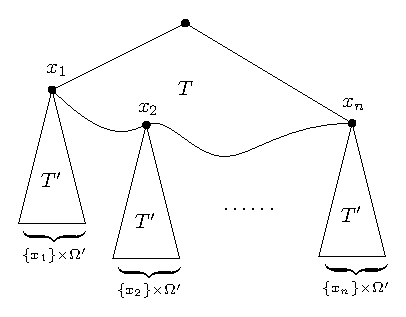
\includegraphics{prefixcodecomposition}
  \caption{The composition of prefix-free codes is prefix-free.}
  \figlabel{prefixcodecomposition}
\end{figure}

Let $C : \Omega \to \{0, 1\}^*$ and $C' : \Omega' \to \{0, 1\}^*$ be
prefix-free codes corresponding to trees $T$ and $T'$. Consider the
code $C \cdot C' : \Omega \times \Omega' \to \{0, 1\}^*$, where
\[
(C \cdot C')(x, y) = C(x) C'(y).
\]
It is easily seen that the tree of \figref{prefixcodecomposition}, in
which each leaf of $T$ is replaced by a copy of $T'$, is the tree
corresponding to $C \cdot C'$. In other words, the composition of
prefix-free codes is prefix-free. We will make use of this fact.

Let $h$ be such that $2^{h - 1} < |\Omega| \leq 2^{h}$, and consider
the complete binary tree of height $h$. If we assign the leftmost
leaves of this tree to the elements of $\Omega$ and discard the
remaining leaves, truncating the tree, we effectively obtain a
prefix-free code $C$ for $\Omega$ for which
\begin{align}
  |C(x)| = h = \ceil{\log |\Omega|}, \eqlabel{fixed-length}
\end{align}
\emph{i.e.}~any finite set $\Omega$ can be given a prefix-free code
for which every codeword has length $\ceil{\log |\Omega|}$. We will
call this the \emph{fixed-length encoding} of $\Omega$. It is
important to note that such a code requires the decoder to know the
size of $\Omega$ to determine the string's delimitations.

\begin{exm}
  In some cases, we are interested in encoding a set of size
  $n!$. Recall Stirling's approximation,
  \[
  n! = \sqrt{2 \pi n} \left(\frac{n}{e}\right)^n e^{r(n)},
  \]
  where $r(n)$ satisfies
  $\frac{1}{12n + 1} < r(n) < \frac{1}{12n}$~\cite{robbins:stirling}.
  We can use this approximation to bound the length of fixed-length
  codes of these sets, so
  \begin{align}
    \log n! & = n \log n - n \log e + \frac{1}{2} \log n + \log \sqrt{2\pi} + \varTheta(1/n)  \notag \\
            & \leq n \log n - n \log e + O(\log n). \eqlabel{perm-code-loose} \enspace
  \end{align}

  Note that such a fixed-length code would have length
  $\ceil{\log n!}$, but we have chosen to ignore the ceiling in this
  analysis for reasons to be made clear later.
\end{exm}

The correspondence between prefix-free codes and binary trees is
useful in proving the next result, which is central to the function of
prefix-free encoding arguments.
\begin{defn}
  A function $\ell : \Omega \to \R$ is said to \emph{satisfy Kraft's
    condition} if
  \[\sum_{x \in \Omega} 2^{-\ell(x)} \leq 1.\]
\end{defn}

\begin{lem}[Kraft's Inequality~\cite{kraft:inequality}]\lemlabel{kraft-inequality}
  If $C : \Omega \to \{0, 1\}^*$ is a prefix-free code, then
  $|C(\cdot)| : \Omega \to \N$ satisfies Kraft's
  condition. Conversely, given some function $\ell : \Omega \to \N$
  satisfying Kraft's condition, there exists a prefix-free code
  $C : \Omega \to \{0, 1\}^*$ for which $|C(x)| = \ell(x)$ for all
  $x \in \Omega$.
\end{lem}
\begin{proof}
  First, consider the tree corresponding to the prefix-free code
  $C$. Let each degree 2 node represent a $\text{Bernoulli}(1/2)$
  random variable, where each one of the left or right children is
  chosen with probability $1/2$; degree 1 nodes automatically choose
  their only child. Let $X$ denote the leaf node obtained by following
  this random process from the root. Then
  \[1 = \Pr\left[\bigcup_{x \in \Omega} (X = x)\right] = \sum_{x \in \Omega} \Pr[X =
  x] \geq \sum_{x \in \Omega} 2^{-|C(x)|},\]
  with equality if and only if each internal node has degree 2.

  Conversely, write $\ell(x_1) \leq \cdots \leq \ell(x_n)$. Consider
  the complete binary tree $T$ of height $\ell(x_n)$. We transform $T$
  into a tree which corresponds to a prefix-free code satisfying
  Kraft's condition.

  Choose a node $u_1$ at depth $\ell(x_1)$ (say, the first encountered
  in a depth first traversal) and remove its subtree from $T$. The
  code $C(x_1)$ will correspond to the root-to-leaf path to
  $u_1$. Continue this process for depths $\ell(x_2)$ through
  $\ell(x_n)$. The only way this process can fail is if the tree has
  no leaves at depth $\ell(x_n)$ at any point. But the number of
  leaves at depth $\ell(x_n)$ before step $j$ in which the code
  $C(x_j)$ is assigned is
  \begin{align*}
    2^{\ell(x_n)} - \sum_{i = 1}^{j - 1} 2^{\ell(x_n) - \ell(x_i)} =
    2^{\ell(x_n)}\left(1 - \sum_{i = 1}^{j - 1} 2^{-\ell(x_i)}\right)
    > 2^{\ell(x_n)}\left(1 - \sum_{i = 1}^n 2^{-\ell(x_i)}\right)
    \geq 0,
  \end{align*}
  so the process completes. If $T$ has any extra leaves which do not
  correspond to elements of $\Omega$, then prune them from the
  tree. The remaining tree $T$ corresponds to a prefix-free code $C$
  for which $|C(x_i)| = \ell(x_i)$ for each $i$.
\end{proof}

It is a fact that \lemref{kraft-inequality} also holds for uniquely
decipherable codes. Therefore, in some sense, we are justified in
restricting our study strictly to prefix-free codes, since for any
uniquely decipherable encoding of a set, there exists a prefix-free
code for the same set with exactly the same codeword
lengths~\cite{gallager:informationtheory,
  mcmillan:uniquedecipherability}.

Suppose now that we are interested in encoding an incremental sequence
of choices for which the number of options at any point depends upon
previous choices. Indeed, we define sets $\Omega_1, \ldots, \Omega_t$
such that $\Omega_1$ is fixed and $\Omega_{i + 1}$ depends on some
sequence of selections $(x_1, \ldots, x_i) \in \Omega_1 \times \cdots
\times \Omega_i$. The set $\Omega_1 \times \cdots \times \Omega_t$ is
called the \emph{decision space} for the sequence of choices $x =
(x_1, \ldots, x_t)$. Suppose that the decision space for $x$ has size
$d$. We can encode $x$ by presenting a sequence of fixed-length
encodings for $x_i \in \Omega_i$, and the code for $x$ then has length
\[
\sum_{i = 1}^t \ceil{\log |\Omega_i|} \leq \log \prod_{i=1}^t
|\Omega_i| + t = \log d + t,
\]
and indeed, each choice may incur an extra bit in the code,
\emph{e.g.}~if $|\Omega_i| = 2^{n} + 1$, then this code has length $nt + t$, but
\[
\log d = \log (2^n + 1)^t = t \log (2^n + 1) \leq nt + O(t 2^{-n}).
\]

The next result, attributed to Jiang, allows us to encode $x$ without
requiring extra bits.
\begin{lem}[Lucier \emph{et al.}~\cite{lucier.jiang.li:quicksort}]\lemlabel{incremental-code}
  If $x$ is an incremental choice of values with a decision space of
  size $d$, then $x$ can be encoded with $\ceil{\log d}$ bits.
\end{lem}
\begin{proof}
  Suppose that $x = (x_1, \ldots, x_t)$ has the decision space
  $\Omega_1 \times \cdots \times \Omega_t$, and let
  $k_i \in \{0, \ldots, |\Omega_i| - 1\}$ be the index of $x_i$ in
  $\Omega_i$, for each $1 \leq i \leq t$. Consider the integer
  \[k = k_1 + k_2 |\Omega_1| + k_3 |\Omega_1| |\Omega_2| + \cdots +
  k_t \prod_{i=1}^{t-1}|\Omega_i|.\] We know that
  \[0 \leq k \leq (|\Omega_1| - 1) + (|\Omega_2| - 1)|\Omega_1| +
  \cdots + (|\Omega_t| - 1)\prod_{i = 1}^{t - 1} |\Omega_i| = d - 1,\]
  since telescoping kills each $\prod |\Omega_i|$ except for the last
  one. So our encoding for $x$ is simply a fixed-length encoding of
  $k$.

  To decode $x = (x_1, \ldots, x_t)$ from the value of $k$, we can
  compute and retrieve $k_1 = k \bmod |\Omega_1|$, since we know
  $|\Omega_1|$. From the value $k_1$, we determine $x_1$, which in
  turn determines $|\Omega_2|$. We can then retrieve $k_2$ from
  $k_2 |\Omega_1| + k_1 = k \bmod |\Omega_2|$, so we determine
  $x_2$. Continuing in this way, we can determine all of
  $x = (x_1, \ldots, x_t)$. From \eqref{fixed-length}, this code has
  length $\ceil{\log d}$.
\end{proof}

This result becomes useful when analyzing constant factors or lower
order terms, or if the number of choices is significant
(\emph{e.g.}~in \secref{records}). In many cases, only a constant
number of choices are made, which causes only at most an insignificant
constant number of wasted bits. Moreover, other approximations in
codeword lengths sometimes involve a super-constant lower order term,
in which case the result is likely useless (\emph{e.g.}~whenever
\eqref{perm-code-loose} is invoked).

\section{Entropy}

Each code $C : \Omega \to \{0, 1\}^*$ has an associated random
variable of codeword lengths $|C(\cdot)| : \Omega \to \N$, which is
our main object of study. The following definition will help to
understand and quantify codeword length optimality.
\begin{defn}
  The \emph{entropy} $\ent(X)$ of a random variable
  $X : \Omega \to \R$ with probability density $p$ is
  \[\ent(X) = \sum_{x \in \Omega} p_x \log \frac{1}{p_x},\]
  sometimes denoted by $\ent(p)$. The \emph{binary entropy function}
  $H : [0, 1] \to \R$ is defined by
  \[H(\alpha) = \ent(\text{Bernoulli}(\alpha)) = \alpha \log
  \frac{1}{\alpha} + (1 - \alpha) \log \frac{1}{1 - \alpha},\]
  where $H(0) = H(1) = 0$.
\end{defn}

In this thesis, we sometimes use the following approximation of the
binary entropy function:
\begin{align}
  H(\alpha) & = \alpha \log \frac{1}{\alpha} + (1 - \alpha) \log \frac{1}{1 - \alpha} \notag \\
  & = \alpha \log \frac{1}{\alpha} + (1 - \alpha) \log \left(1 + \frac{\alpha}{1 - \alpha}\right) \notag \\
  & \leq \alpha \log \frac{1}{\alpha} + \alpha \log e = \alpha \log
  (e/\alpha), \eqlabel{entropy-approx}
\end{align}
since $1 + x \leq e^x$ for every $x \in \R$. See
\figref{entropy-approx-plot} for a comparison between $H(\alpha)$ and
its approximation.

\begin{figure}
  \centering
  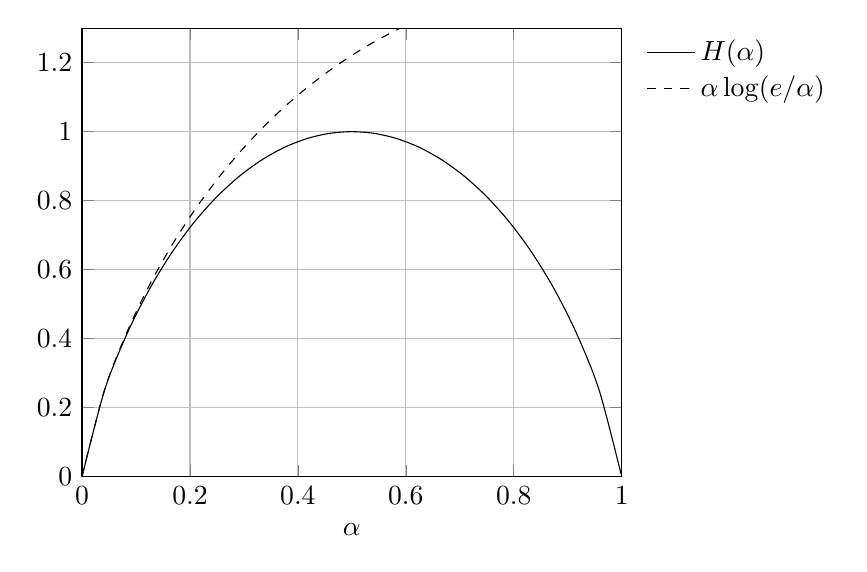
\begin{tikzpicture}
    \begin{axis}[
      xlabel=$\alpha$,
      legend cell align=left,
      legend pos=outer north east,
      legend style={draw=none},
      grid=major,
      ymin=0,
      ymax=1.3,
      xmin=0,
      xmax=1
      ]

      \addplot[
      smooth,
      domain=0:1
      %blue
      ]
      {-x*log2(x) - (1 - x)*log2(1 - x)};
      \addlegendentry{$H(\alpha)$}
    
      \addplot[
      smooth,
      domain=0:1,
      style=dashed
      %color=red
      ]
      {-x*log2(x) + x*log2(e)};
      \addlegendentry{$\alpha \log (e/\alpha)$}
    \end{axis}
  \end{tikzpicture}
  \caption{Comparison between $H(\alpha)$ and its approximation from
    \eqref{entropy-approx}.}
  \figlabel{entropy-approx-plot}
\end{figure}

We will see how the entropy of $X$ describes the expected amount of
information in bits required to represent $X$. Consider the following
examples:
\begin{exm}
  Let $X : \{1, \ldots, n\} \to \R$ be uniformly distributed. From
  \eqref{fixed-length}, we can encode each element of
  $\{1, \ldots, n\}$ with a fixed-length code of length
  $\ceil{\log n}$. Moreover, we easily see that $\ent(X) = \log n$.
\end{exm}

\begin{exm}
  Let $X : \{1, \ldots, n\} \to \R$ have probability density
  $p_i = 1/2^i$ for $1 \leq i < n$, and $p_n = 1/2^{n - 1}$. Then
  \[\lim_{n \to \infty} \ent(X) = 2.\]

  This is a dramatic difference in entropy from the previous example,
  demonstrating that a fixed-length code for $X$ would be terribly
  inefficient, since several elements of $X$ appear with exponentially
  low probability. In this case, a more judicious coding strategy is
  required. Consider the code $C$ such that
  \[
  C(i) = \left\{
  \begin{array}{ll}
    0^{i - 1} \; 1 & \mbox{if $1 \leq i < n$};\\
    0^{n - 1} & \mbox{if $i = n$}.
  \end{array} \right.
  \]
  Notice that this code is prefix-free with expected codeword length
  exactly $\ent(X)$.
\end{exm}

We can prove that $\log (1/p_x)$ is the optimal codeword length for
any element $x \in \Omega$. We rely on the following classic result.
\begin{thm}[Jensen's Inequality]\thmlabel{jensen}
  For any concave function $f$ and any random variable $X$,
  \[
  \E[f(X)] \leq f(\E[X]) .
  \]
  This inequality is reversed if $f$ is convex.
\end{thm}
\begin{thm}\thmlabel{optimal-kraft}
  If $\ell : \Omega \to \R$ satisfies Kraft's condition, where
  $\Omega$ is endowed with the probability density $p$, then
  \[
  \sum_{x \in \Omega} p_x \log (1/p_x) = \ent(p) \leq \E[\ell(x)] = \sum_{x \in \Omega} p_x \ell(x) .
  \]
\end{thm}
\begin{proof}
  We examine the value $\ent(p) - \E[\ell(x)]$, where
  \begin{align}
    \ent(p) - \E[\ell(x)] &= \sum_{x \in \Omega} p_x \log (1/p_x) - \sum_{x \in \Omega} p_x \ell(x) \notag \\
                          &= \sum_{x \in \Omega} p_x \log \left(\frac{2^{-\ell(x)}}{p_x}\right) \notag \\
                          &= \E\left[\,\log \left(\frac{2^{-\ell(x)}}{p_x}\right)\,\right] \notag \\
                          &\le \log \left(\E\left[\,\frac{2^{-\ell(x)}}{p_x}\,\right]\right), \eqlabel{entropy-optimal}
  \end{align}
  by Jensen's inequality, since $\log$ is a concave function. Then,
  \eqref{entropy-optimal} becomes
  \[
  \log \left(\E\left[\,\frac{2^{-\ell(x)}}{p_x}\,\right]\right) = \log
  \left( \sum_{x \in \Omega} 2^{-\ell(x)} \right) \le \log 1 = 0
  \]
  by \lemref{kraft-inequality}.
\end{proof}
Shannon proved the following result, which describes how entropy
relates to codeword lengths; in addition to satisfying the conditions
of the previous theorem, codeword lengths must also be integers.
\begin{thm}[Noiseless Coding Theorem~\cite{shannon:mathematical}]\thmlabel{noiseless-coding}
  If $C : \Omega \to \{0, 1\}^*$ is a prefix-free code with
  probability density $p$ minimizing its expected codeword length,
  then
  \[\ent(p) \leq \E\left[\,|C(x)|\,\right] < \ent(p) + 1.\]
\end{thm}

%In this sense, $\log (1/p_x)$ is the optimal codeword length for any
%element $x \in \Omega$, since
%$\E\left[\,|C(x)|\,\right] = \sum_{x \in \Omega} p_x |C(x)|$, and
%$\ent(p) = \sum_{x \in \Omega} p_x \log (1/p_x)$. In fact, it can be
%shown through standard optimization techniques that for any
%(potentially non-integer valued) function $\ell : \Omega \to \R$
%satisfying Kraft's condition and any probability density
%$p : \Omega \to [0, 1]$, the minimum value of
%$\sum_{x \in \Omega} p_x \ell(x)$ is attained when
%$\ell(x) = \log (1/p_x)$, so that
%\[\sum_{x \in \Omega} p_x \ell(x) = \ent(p).\]

\section{Shannon-Fano Codes}

Earlier, we showed how to encode the set $\Omega$ using a fixed-length
code. Suppose now that $\Omega$ is augmented with a probability
distribution. Our goal is to provide a better code, in the sense that
more probable elements are given appropriately shorter codes.

The \emph{Shannon-Fano code} for $\Omega$ is a prefix-free code
constructed from a probability distribution over the elements of
$\Omega$~\cite{fano:transmission, shannon:mathematical}.

%More specifically, the algorithm constructs a
%full binary tree with the elements of $X$ as its leaves, and the
%encoding is understood from this tree.

Let $\Omega$ be endowed with the probability density $p$. Since
\[\sum_{x \in \Omega} 2^{-\ceil{\log (1/p_x)}} \leq \sum_{x \in \Omega} 2^{-\log
  (1/p_x)} = \sum_{x \in \Omega} p_x = 1,\]
then the proof of \lemref{kraft-inequality} gives a deterministic
construction for a prefix-free code $C : \Omega \to \{0, 1\}^*$, where
\[
|C(x)| = \Ceil{\log \frac{1}{p_x}}. \eqlabel{shannon-fano-optimality}
\]
This is the Shannon-Fano code: see \figref{shannon-fano} for an
example construction.

%This specific code is the Shannon-Fano
%code.
%
%The Shannon-Fano code $C(x_i)$ for
%$x_i$ will be shown to have length:
%\[|C(x_i)| = \ceil{\log (1/p_{x_i})}\]
%
%Indeed, by \lemref{kraft-inequality}:
%\[\sum_{x \in X} 2^{-|C(x)|} \leq \sum_{x \in X} 2^{-\log (1/p_x)} =
%\sum_{x \in X} p_x = 1\]
%
%so a prefix-free code with such codeword lengths does exist, and it is
%described by the construction given in the proof of
%\lemref{kraft-inequality}.

\begin{figure}
  \centering
  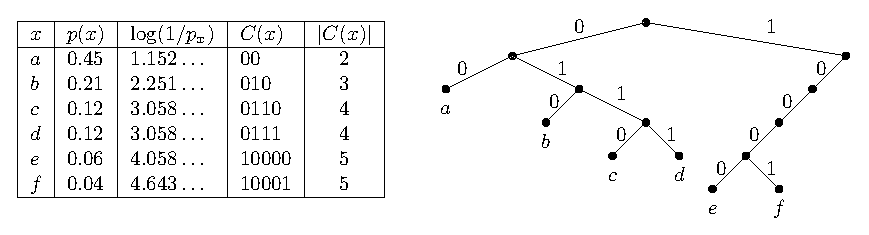
\includegraphics{shannon-fano}
  \caption{The Shannon-Fano code and corresponding tree for a set and
    probability distribution as given by the construction in
    \lemref{kraft-inequality}. Notice the values $\log (1/p_x)$ and
    $|C(x)|$.}
  \figlabel{shannon-fano}
\end{figure}

A useful fact about the codes presented in this section is that they
are locally optimal in the sense of \thmref{noiseless-coding}, since
the optimal codeword length for $x \in \Omega$ is $\log (1/p_x)$.
Local optimality will prove to be more useful to us than global
optimality.

Note that if we choose $p$ to be the uniform distribution, then
$p_x = 1/|\Omega|$, and the Shannon-Fano code $C$ for $\Omega$ is such
that
\[
|C(x)| = \ceil{\log |\Omega|},
\]
as seen previously with \eqref{fixed-length}.

We will mostly apply Shannon-Fano codes in the encoding of random bit
strings $x = x_1 \cdots x_n$, where all $x_i$ are independent and
identically distributed as $\text{Bernoulli}(p)$ random variables. We
will say that $p$ is the \emph{parameter} for this Shannon-Fano
code. Let $n_1(x)$ denote the number of one bits in $x$, and $n_0(x) =
n - n_1(x)$ denote the number of zero bits in $x$. Then, a particular
string $x$ appears with probability exactly $p^{n_1(x)} (1 -
p)^{n_0(x)}$. In this case, the codeword for $x$ has length
\[|C(x)| = \left\lceil n_1(x) \log \frac{1}{p} + n_0(x) \log
  \frac{1}{1 - p} \right\rceil.\]

\begin{exm}
  We are often concerned with producing fixed-length encodings for
  sets of size ${n \choose k}$. Since
  \[
  \left(\frac{k}{n}\right)^k \left(1 - \frac{k}{n}\right)^{n - k} =
  2^{-n H(k/n)}
  \]
  is the probability that a particular $n$-bit binary string with
  exactly $k$ ones appears if each bit is chosen with probability
  $k/n$, then the Shannon-Fano code with parameter $k/n$ for this bit
  string has length $\lceil n H(k/n) \rceil$. Since the number of bit
  strings of length $n$ containing exactly $k$ ones is $\binom{n}{k}$,
  then
  \[
  \log \binom{n}{k} \leq \lceil n H(k/n) \rceil,
  \]
  establishing a bound on the length of fixed-length encodings for
  such sets---in fact, using \thmref{optimal-kraft} we can show that
  this ceiling can be omitted, and
  \begin{align}
    \log \binom{n}{k} \leq n H(k/n). \eqlabel{binom-code-tight}
  \end{align}
  %Again, from
  %\thmref{stirling} and \eqref{perm-code-tight} we see that
  %\begin{align}
  %  \log {n \choose k} & = \log n! - \log k! - \log (n - k)! \notag \\
  %                     & = n \log n - k \log k - (n - k) \log (n - k) + \frac{1}{2} \log \frac{n}{k(n - k)} + \varTheta(1/k) \notag \\
  %                     & \leq k(\log n - \log k) + (n - k) (\log n - \log (n - k)) + O(1) \notag \\
  %                     & = n H(k/n) + O(1).  \eqlabel{binom-code-tight}
  %\end{align}
  Applying the estimate from \eqref{entropy-approx}, we obtain that
  \begin{align}
    \log {n \choose k} \leq k \log n - k \log k + k \log e. \eqlabel{binom-code-loose}
  \end{align}
  This estimate is only useful when $k/n$ is small.  We can instead
  obtain a similar and slightly worse bound than
  \eqref{binom-code-tight} by relying on Stirling's approximation and
  the fact that $\binom{n}{k} = \frac{n!}{k!(n - k)!}$.
\end{exm}

We give an example of when it might be more useful to apply
\eqref{binom-code-tight} over \eqref{binom-code-loose}: suppose we
wish to encode a sparse bit string, \emph{i.e.}~a bit string in which
$n_1(x)$ is relatively small.
\begin{lem}\lemlabel{bitstring-compression}
  Let $x \in \{0, 1\}^n$, where $n_1(x) \leq \alpha n$ for some
  $0 \leq \alpha \leq 1/2$. Then, we can give a prefix-free code for
  $x$ of length at most $\log n + n H(\alpha) + O(1)$.
\end{lem}
\begin{proof}
  Encode $x$ by giving the value $n_1(x)$, and then the set of
  positions of the $n_1(x)$ ones in the string. This allows us to
  deduce the entire bit string. Since $n_1(x) \leq \alpha n$ and
  $0 \leq \alpha \leq 1/2$, then
  ${n \choose n_1(x)} \leq {n \choose \alpha n}$, so our code has
  length at most
  \[\log n + n H(\alpha) + O(1). \qedhere\]
\end{proof}

In this case, \eqref{binom-code-tight} grants us immediate higher
order savings for any $0 \leq \alpha < 1/2$ over the trivial encoding
of $x$, since $H$ is strictly increasing on $[0, 1/2]$, and since
$H(1/2) = 1$. If instead \eqref{binom-code-loose} were used, savings
would only be obtained for $\alpha \geq 0$ satisfying $\alpha \log
\frac{1}{\alpha} + \alpha \log e < 1$, \emph{i.e.}~$\alpha <
0.32756...$.

\section{Elias Codes}\seclabel{elias}

We have so far only explicitly discussed encodings for finite sets. In
this section, we present a preliminary set of prefix-free codes
developed by Elias~\cite{elias:coding} and used to encode the set of
natural numbers. Indeed, we are only ever concerned with encoding
positive integer values: once an ordering for a set $\Omega = \{x_1,
x_2, \ldots \}$ is established, we can encode the element $x_i$ by
giving the value $i \in \N$.

Let $i \geq 1$ be the subject of our encoding. Let $s_i$ be the binary
representation of $i$, so $|s_i| = \floor{\log i} + 1$. The
\emph{Elias $\gamma$-code} for $i$ is then
\[E_\gamma(i) = 0^{|s_i| - 1} \; s_i,\]
of length $|E_\gamma(i)| = 2|s_i| - 1 = 2 \floor{\log i} + 1$. Note
that $s_i$ begins with a one. To decode $E_\gamma(i)$ and recover the
value $i$, we read the code from left to right. If $n$ zeroes are
observed before the first one, then the next $n + 1$ bits represent
$s_i$, from which we obtain $i$.

The \emph{Elias $\delta$-code} will prove to be more useful to us. As
before, let $s_i$ be the binary representation of $i$, and
$|s_i| = \floor{\log i} + 1$. Note that $|s_i| \geq 1$. The code is
\[E_\delta(i) = E_\gamma(|s_i|) \; s_i',\]
where $s_i'$ is the string $s_i$ minus its leading bit, which is
always a one. Thus
\begin{align*}
  |{E_\delta}(i)| & = |{E_\gamma}(|s_i|)| + |s_i| - 1 = \floor{\log i} + 2
                  \floor{\log (\floor{\log i} + 1)} + 1 \\
                & \leq \log i + O(\log \log i).
\end{align*}
To decode $E_\delta(i)$, we read it from left to right, and encounter
the self-delimiting code $E_\gamma(|s_i|)$ which tells us the value of
$|s_i|$. From this, we then know that the remaining $|s_i| - 1$ bits
form the truncated binary representation of $i$.

Finally, in some cases we may wish to use the \emph{Elias
  $\omega$-code}, which is the recursive variant of the previous
scheme. As before, let $s_i$ be the binary representation of $i$. The
$\omega$-code is
\[
E_\omega(i) = \left\{
  \begin{array}{ll}
    \widetilde{E}_\omega(|s_i| - 1) \; s_i \; 0 & \mbox{if $i \neq 1$};\\
    0 & \mbox{if $i = 1$},
  \end{array} \right.
\]
where
\[
\widetilde{E}_\omega(i) = \left\{
  \begin{array}{ll}
    \widetilde{E}_\omega(|s_i| - 1) \; s_i & \mbox{if $i \neq 1$};\\
    \epsilon & \mbox{if $i = 1$}.
  \end{array} \right.
\]
To decode the string $E_\omega(i)$, we read it from left to right
according to the following procedure:
\begin{enumerate}
\item If $E_\omega(i) = 0$, then return $1$;
\item Let $k \leftarrow 1$, and point to the leftmost bit of
  $E_\omega(i)$;
\item The next $k + 1$ bits represent some integer $n$;
\item If the next bit is a zero, then return $n$. If not, go to step 3
  with $k \leftarrow n$.
\end{enumerate}
The Elias $\omega$-code has length
\begin{align*}
  |E_\omega(i)| & = 2 + \floor{\log i} + |\widetilde{E}_\omega(\floor{\log i})| \\
                & = 3 + \floor{\log i} + \floor{\log \floor{\log i}} + |\widetilde{E}_\omega(\floor{\log \floor{\log i}})| \\
                & \leq \log i + \log \log i + \log \log \log i + \cdots + \underbrace{\log \cdots \log}_{\text{$\log^* i$ times}} i + O(\log^* i),
\end{align*}
where $\log^* i$ is the slowly growing iterated logarithm function,
defined by
\[
\log^* i = \left\{
  \begin{array}{ll}
    1 + \log^*(\log i) & \mbox{if $i > 1$};\\
    0 & \mbox{if $i \leq 1$}.
  \end{array} \right.
\]

\begin{figure}
  \centering
  \begin{tabular}{| l | l | l | l | l |}
    \hline
    $i$ & $s_i$ & $E_\gamma(i)$ & $E_\delta(i)$ & $E_\omega(i)$ \\ \hline
    $1$ & $1$ & $1$ & $1$ & $0$ \\ %\hline
    $2$ & $10$ & $010$ & $010 0$ & $100$\\ %\hline
    $3$ & $11$ & $011$ & $010 1$ & $110$\\ %\hline
    $4$ & $100$ & $00100$ & $011 00$ & $101000$ \\ %\hline
    $5$ & $101$ & $00101$ & $011 01$ & $101010$ \\ %\hline
    $66$ & $1000010$ & $0000001000010$ & $00111000010$ & $1011010000100$ \\
    $67$ & $1000011$ & $0000001000011$ & $00111000011$ & $1011010000110$ \\
    $68$ & $1000100$ & $0000001000100$ & $00111000100$ & $1011010001000$ \\ 
    $69$ & $1000101$ & $0000001000101$ & $00111000101$ & $1011010001010$ \\
    $70$ & $1000110$ & $0000001000110$ & $00111000110$ & $1011010001100$ \\ \hline
  \end{tabular}
  \caption{Some Elias codes for small integers.}
  \figlabel{elias-codes}
\end{figure}

Elias also proved that his $\delta$-codes and $\omega$-codes are
asymptotically optimal in the sense of \thmref{noiseless-coding}.
\begin{prop}
  If $i \in \{1, \ldots, n\}$ is chosen according to the probability
  density $p$, where $p_{1} \geq \cdots \geq p_{n}$, then
  \[
  \lim_{\ent(p) \to \infty} \frac{\E\left[\,|E_\gamma(i)|\,\right]}{\ent(p)} = 2
  \]
  and
  \[
  \lim_{\ent(p) \to \infty} \frac{\E\left[\,|E_\delta(i)|\,\right]}{\ent(p)} = \lim_{\ent(p) \to \infty} \frac{\E\left[\,|E_\omega(i)|\,\right]}{\ent(p)} = 1 .
  \]
  %\[
  %\frac{\E\left[\,|E_\delta(i)|\,\right]}{\ent(p)}, \frac{\E\left[\,|E_\omega(i)|\,\right]}{\ent(p)}  \to 1\]
\end{prop}

See \figref{elias-codes} for a comparison between the codes developed
in this section.

\section{Kolmogorov Complexity}\seclabel{k-complexity}

Encoding arguments have largely been studied through the lens of
Kolmogorov complexity. We present a brief overview of the theory of
Kolmogorov complexity and its central results. See the books by Li and
Vit\'{a}nyi~\cite{li.vitanyi:introduction}, or Cover and Thomas for a
more in-depth introduction~\cite{thomas:elements}.

Informally, the Kolmogorov complexity of a bit string $x$ is the
length of a ``shortest effective binary description'' for $x$, first
proposed independently by Kolmogorov, Solomonoff, and
Chaitin~\cite{chaitin:intro, kolmogorov:complexity,
  solomonoff:intro}. This notion of effectiveness, in the end,
subsumes a model of computation.

Consider for example the following bit strings:
\begin{align}
  &111001000101100101011000; \eqlabel{k-example-1}\\
  &101010101010101010101010. \eqlabel{k-example-2}
\end{align}

There does not appear to be a concise way of describing
\eqref{k-example-1}, rather than simply giving the string itself. In
other words, this string appears to be highly random. The string
\eqref{k-example-2}, however, exhibits clear regularity, and can be
described by a program which is instructed to print the string `$10$'
twelve times. Such a program has length $O(\log n)$, if $n$ is the
length of the given bit string---exponentially less than the length of
the description for \eqref{k-example-1}, a ``random'' string.

The Kolmogorov complexity $K(x)$ of a string $x$ is the length of the
shortest program in binary which outputs $x$ and halts, in some fixed
language. Formally, we fix a universal Turing machine $U$.

\begin{defn}
  The \emph{Kolmogorov complexity} of $x \in \{0, 1\}^n$ is
  \[K_U(x) = \min \{ |p| : U(p) = x\}.\]
\end{defn}

Conveniently, the following well-known result indicates that our
choice of universal Turing machine does not matter.
\begin{thm}[Universality of Kolmogorov Complexity]
  For any $x \in \{0, 1\}^n$ and for any universal Turing machines
  $U, A$, we have that
  \[K_U(x) \leq K_A(x) + O(1).\]
\end{thm}

Thus, we disregard the specification of $U$ and always speak of $K(x)$
with some loose constant term in mind.

Unsurprisingly, Kolmogorov complexity is related to entropy in a kind
of law of large numbers.
\begin{thm}
  If $x_1, \ldots, x_n$ are independent and identically distributed
  $\text{Bernoulli}(p)$,
  \[\lim_{n \to \infty} \frac{\E[K(x_1 \cdots x_n)]}{n} =
  H(p).\]
\end{thm}

The discussion of Kolmogorov complexity surrounding
\eqref{k-example-1} and \eqref{k-example-2} describes one of the
central concepts in the study of encoding arguments through Kolmogorov
complexity. By saying that no concise description of
\eqref{k-example-1} exists, we essentially said that it is
\emph{incompressible}. The following result says that the overwhelming
majority of strings are incompressible:
\begin{thm}[Incompressibility Theorem]\thmlabel{incompressibility}
  If $x \in \{0, 1\}^n$ is chosen uniformly at random, then for any
  $s \geq 0$,
  \[\Pr[K(x) \leq n - s] \leq 2^{-s}.\]
\end{thm}

These results establish most of the background necessary to develop
encoding arguments via Kolmogorov complexity. In such an argument, we
are interested in bounding the probability of some event happening. We
choose an object at random---when the event in question occurs, we can
describe the object concisely, and it becomes compressible. From the
previous result, the random object should be largely incompressible
with high probability, so we obtain a bound on the probability of the
given event.

\chapter{Uniform Encoding and Applications}\chlabel{uel}
The partial prefix-free codes designed and studied in this chapter
will all be denoted $C : \Omega \to \{0, 1\}^* \cup \{\bot\}$, where
$\Omega$ is to be understood from context.

\section{The Uniform Encoding Lemma}

\begin{lem}\lemlabel{uel}
  Let $C : \Omega \to \{0, 1\}^* \cup \{\bot\}$ be a partial
  prefix-free code. Let $x \in \Omega$ be chosen uniformly at
  random. Then, for any $s \geq 0$,
  \[\Pr\left[\,|C(x)| \leq \log |\Omega| - s\,\right]
  \leq 2^{-s}.\]
\end{lem}
\begin{proof}
  Recall that we chose $|\bot| = \infty$, so if
  $C(x) \leq \log |\Omega| - s$, then $C(x)$ is defined.
  %Since $C$ is
  %bijective, then uniform selection of $x \in \Omega$ implies uniform
  %selection of $C(x)$ among all codewords of $C$.
  Let $k = \log |\Omega| - s$. Since $C$ has $|\Omega|$ codewords, and
  at most $2^k$ of those have length at most $k$, then the probability
  that $C(x)$ has length at most $k$ is at most
  \[\frac{2^{k}}{|\Omega|} = \frac{2^{\log |\Omega| - s}}{|\Omega|} =
  \frac{1}{2^s}. \qedhere\]
\end{proof}

This lower tail inequality is analogous to \thmref{incompressibility}
and is similarly crucial in proving results through encoding. The
approach is virtually the same as that described in
\secref{k-complexity}---only now, the length of an effective
description of an object is the length of its corresponding
prefix-free code.

For example usage of \lemref{uel}, see the proof of
\propref{binary-runs}.

\section{Permutations and Binary Search Trees}

\begin{defn}
  %A \emph{permutation} of size $n$ is a bijection
  %$\sigma : \{1, \ldots, n\} \to \{1, \ldots, n\}$, sometimes denoted
  %\[\sigma = (\sigma(1), \ldots, \sigma(n)).\]
  %The number of distinct permutations of size $n$ is $n!$.
  %is a sequence of $n$
  A \emph{permutation} $\sigma$ of size $n$ is a sequence of $n$
  distinct integers, sometimes denoted
  \[\sigma = (\sigma(1), \ldots, \sigma(n)).\]
  Except when explicitly stated, we will assume that the set of
  integers involved in a permutation of size $n$ is precisely
  $\{1, \ldots, n\}$. The number of such permutations is $n!$.
\end{defn}

%\subsection{Longest Ascending Run}
%
%\begin{defn}
%  For a permutation $\sigma$ of size $n$, an \emph{ascending run} of
%  length $k$ is a tuple
%  $(\sigma(i_1), \sigma(i_2), \ldots, \sigma(i_k))$ where
%  $1 \leq i_1 < \cdots < i_k \leq n$ and
%  $\sigma(i_1) < \cdots < \sigma(i_k)$.
%\end{defn}
%
%The length of the longest ascending run in a random permutation has
%been well-studied. Logan and Shepp~\cite{logan.shepp:runs} together
%with Vershik and Kerov~\cite{vershik.kerov:runs} are the first who
%established that the expected length of the longest ascending run in a
%random permutation is asymptotically $2\sqrt{n}$. Several new original
%proofs of this fact have appeared more recently; accordingly, we
%present an encoding argument to study this problem.
%
%\begin{thm}
%  Let $\sigma$ be a uniformly random permutation of size $n$. Then,
%  the longest ascending run in $\sigma$ has length at most
%  $(e + o(1))\sqrt{n}$ with probability $1 - O(1/n)$.
%\end{thm}
%\begin{proof}
%  We encode a permutation $\sigma$, which is chosen uniformly at
%  random from a set of size $n!$.
%
%  Suppose that $\sigma$ has an ascending run of length $t$. We encode
%  $\sigma$ by providing the set of values in this run; then the
%  indices in which they appear; and finally, the rest of the
%  permutation. Therefore,
%  \begin{align}
%    |C(\sigma)| &\leq 2 \log {n \choose t} + \log (n - t)! + O(1) \notag \\
%                &= \log n! + 2 \log {n \choose t} - \sum_{0 \leq i < t} \log (n - i) + O(1) \notag \\
%                &\leq \log n! + 2 t \log n - 2t \log t + 2t \log e - \sum_{0 \leq i < t} \log (n - i) + O(1) \tag{by \eqref{binom-code-loose}} \\
%                &\leq \log n! + t \log n - 2t \log t + 2t \log e + t \log \left(1 + \frac{t}{n - t} \right) + O(1) \notag \\
%                &\leq \log n! - 2t \log (t/e\sqrt{n}) + \frac{t^2}{n - t} \log e +
%                  O(1), \eqlabel{ascending-run-part}
%  \end{align}
%  where this last inequality follows since $1 + x \leq e^x$ for all $x
%  \in \R$. Choose $t = \ceil{e\sqrt{n} + (1/2)\ln n}$. Note that $t
%  \leq n/2$ for sufficiently large $n$, so $n - t \geq n/2$ and
%  \[
%  \frac{t^2}{n - t} \leq 2\left(e + \frac{\ln n}{2\sqrt{n}} + O(1/\sqrt{n})\right)^2
%  = O(1),
%  \]
%  so \eqref{ascending-run-part} becomes
%  \begin{align*}
%    |C(\sigma)| &\leq \log n! - 2 \left(e\sqrt{n} + \frac{1}{2}\ln n\right) \log \left(1 + \frac{\ln n}{2e\sqrt{n}}\right) + O(1) \\
%                &\leq \log n! - 2 e \sqrt{n}\log \left(1 + \frac{\ln
%                  n}{2e\sqrt{n}}\right) + O(1).
%  \end{align*}
%  Applying \lemref{uel}, we obtain that $\sigma$ has an ascending run
%  of length $e \sqrt{n} + (1/2)\ln n$ with probability
%  \[O\left(\left(1 + \frac{\ln
%        n}{2e\sqrt{n}}\right)^{-2e\sqrt{n}}\right) = O(e^{-\ln
%    n}) = O(1/n). \qedhere\]
%\end{proof}


\subsection{Records}\seclabel{records}

\begin{defn}
  A \emph{(max) record} in a permutation $\sigma$ of size $n$ is some
  value $\sigma(i)$ with $1 \leq i \leq n$ such that $\sigma(i) =
  \max\{\sigma(1), \ldots, \sigma(i)\}$.
\end{defn}

It is easy to see that the probability that $\sigma(i)$ is a record is
exactly $1/i$, so the expected number of records in a uniformly random
permutation is
\[H_n = \sum_{i = 1}^n \frac{1}{i} = \ln n + O(1),\] the
$n$\textsuperscript{th} harmonic number. It is harder to establish
concentration with non-negligible probability. To do this, one first
needs to show the independence of certain random variables, which
quickly becomes tedious. We instead give an encoding argument to show
concentration of the number of records inspired by a technique used by
Lucier \emph{et al.}~to study the height of random binary search
trees~\cite{lucier.jiang.li:quicksort}.

First, we describe an incremental and recursive manner of encoding a
permutation $\sigma$: begin by providing the first value of the
permutation $\sigma(1)$; followed by the indices of the permutation
for which $\sigma$ takes on a value strictly smaller than $\sigma(1)$,
including an explicit encoding of the induced permutation on the
elements at those indices; and a recursive encoding of the permutation
induced on the elements strictly larger than $\sigma(1)$.

If $\sigma$ contains $k$ elements strictly smaller than $\sigma(1)$,
then the size $S$ of the decision space above satisfies the recurrence
\[S(n) = n \binom{n - 1}{k} k! \cdot S(n - k - 1),\]
with $S(0) = 1$ and $S(1) = 1$. This solves to $S(n) = n!$, so the
encoding described above is no better than a fixed-length encoding for
$\sigma$.

We can readily modify the encoding above to obtain a result about the
concentration of records in a random permutation.

\begin{thm}\thmlabel{records}
  A uniformly random permutation of size $n$ has at least $c \log n$
  records with probability at most
  \[2^{-c (1 - H(1/c)) \log n + O(\log \log n)},\]
  for $c > 2$.
\end{thm}
\begin{proof}
  We encode a permutation $\sigma$ chosen uniformly at random from a
  set of size $n!$.

  Suppose that $\sigma$ has $t \geq c\log n$ records $r_1 < r_2 <
  \cdots < r_t$, for some fixed $c > 2$. First, give a bit string $x =
  x_1 \cdots x_t \in \{0, 1\}^t$, where $x_i = 0$ if and only if $r_i$
  lies in the first half of the interval $[r_{i - 1}, n]$. It follows
  that $n_1(x) \leq \log n$.
%Let $d_i$ denote the number of values of $\sigma$
  %which are greater than $r_i$. If $x_i = 1$, then
  %\[d_{i + 1} \leq (1/2) d_i,\]
  %and therefore,
  %\[1 \leq (1/2)^{n_1(x)} n \iff n_1(x) \leq \log n.\]
  In other words, $x$ is a sparse bit string, and $n_1(x)/t \leq 1/c$.

  To begin our encoding of $\sigma$, we encode the bit string $x$ by
  giving the set of $n_1(x)$ ones in $x$; followed by the incremental
  recursive encoding of $\sigma$ from earlier. In this case, our
  knowledge of the value of $x_i$ halves the size of the space of
  options for encoding the record $r_i$. In other words, our knowledge
  of $x$ allows us to encode each record using roughly one less bit
  per record. More precisely, since the encoding from above recurses
  $t$ times on decreasing values $n_1 > \cdots > n_t$, then the number
  of bits spent encoding records is at most
  \begin{align*}
    \sum_{i = 1}^t \log \lceil n_i/2 \rceil &\leq \sum_{i = 1}^t \log (n_i/2 + 1)
                                              \leq \sum_{i = 1}^t \log (n_i/2) + \sum_{i = 1}^t O(1/n_i) \\
                                            &\leq \sum_{i = 1}^t \log (n_i/2) + H_t = \sum_{i = 1}^t \log n_i - t + O(\log \log n).
  \end{align*}
  Thus, by \lemref{incremental-code}, the total length of the code is
  \begin{align*}
    |C(\sigma)| &\leq \binom{t}{n_1(x)} + \log n! - t + O(\log \log n) \\
                &\leq \log n! - t (1 - H(n_1(x)/t)) + O(\log \log n) \tag{by \eqref{binom-code-tight}}\\
                &\leq \log n! - c (1 - H(1/c))\log n + O(\log \log n).
  \end{align*}
  This last inequality holds since the function $x H(a/x)$ has
  derivative
  \[
  \frac{d}{d x} x H(a/x) = \log \frac{1}{1 - a/x},
  \]
  which is positive as long as $0 < a/x < 1$, and so increases as a
  function of $x$. Applying \lemref{uel}, we obtain the desired
  result.
  %has at most $c \log n$ records with probability $1 - O(1/n)$ for
  %$c \geq 2$ satisfying
  %\[c (1 - H(1/c)) \geq 1.\]
  %A computer-aided calculation shows that $c = 4.40349...$ is the
  %minimal solution to this inequality.
\end{proof}

\subsection{Tree Height}\seclabel{height}

Every permutation $\sigma$ determines a binary search tree
$\text{BST}(\sigma)$ created through the sequential insertion of the
keys $\sigma(1), \ldots, \sigma(n)$. Specifically, if $\sigma_L$
(respectively, $\sigma_R$) denotes the permutation of elements
strictly smaller (respectively, strictly larger) than $\sigma(1)$,
then $\text{BST}(\sigma)$ has $\sigma(1)$ as its root, with
$\text{BST}(\sigma_L)$ and $\text{BST}(\sigma_R)$ as left and right
subtrees. For any $\sigma$, the value $\sigma(1)$ is called its pivot.

Lucier \emph{et al.}~\cite{lucier.jiang.li:quicksort} use an encoding
argument via Kolmogorov complexity to study the height of
$\text{BST}(\sigma)$. They show that for a uniformly chosen
permutation $\sigma$, the tree $\text{BST}(\sigma)$ has height at most
$c \log n$ with probability $1 - O(1/n)$ for $c = 15.498...$; we can
extend our result on records to obtain a tighter result.

For a node $u$, let $s(u)$ denote the number of nodes in the tree
rooted at $u$. Then, $u$ is called balanced if $s(u_L), s(u_R) >
s(u)/4$, where $u_L$ and $u_R$ are the left and right subtrees of $u$
respectively. In other words, a node is said to be balanced if it
occurs in the middle half of its subrange. See
\figref{binary-insertion-tree}.

\begin{figure}
  \centering
  \begin{forest}
    [
    [$10$, for tree={draw,circle,text height=1.5ex,text depth=.25ex,l sep=0.5cm,s sep=1cm,inner sep=0.1cm}
      [$3$
        [$1$
          [,.phantom]
          [$2$]
        ]
        [$7$
          [$5$
            [$4$]
            [$6$]
          ]
          [$9$
            [$8$]
            [,.phantom]
          ]
        ]
      ]
      [$12$
        [$11$]
        [$13$]
      ]
    ]
    ]
  \end{forest}

  \caption{The tree $\text{BST}(\sigma)$, where $\sigma = (10, 12, 3,
    7, 1, 2, 5, 11, 9, 6, 13, 4, 8)$. $\sigma$ has records $10, 12,
    13$. The nodes $5, 7, 12$ are balanced.}
  \figlabel{binary-insertion-tree}
\end{figure}

\begin{thm}\thmlabel{bst-height}
  Let $\sigma$ be a uniformly random permutation of size $n$. Then,
  $\text{BST}(\sigma)$ has height $O(\log n)$ with high probability.
\end{thm}
\begin{proof}
  Suppose that the tree $\text{BST}(\sigma)$ has a rooted path $Y =
  y_1 \cdots y_t$ of length $t \geq c \log n$ for some fixed $c >
  2/\log (4/3)$.

  Our encoding for $\sigma$ has two parts. The first part includes an
  encoding of the value $y_t$, and a bit string $x = x_1 \cdots x_t$,
  where $x_i = 1$ if and only if $y_i$ is balanced. From our
  definition, if $y_i$ is balanced, then
  \[s(y_{i + 1}) \leq (3/4) s(y_i),\]
  and since $n_1(x)$ counts the number of balanced nodes along $Y$,
  then
  \[1 \leq (3/4)^{n_1(x)} n \iff n_1(x) \leq \log_{4/3} n.\]

  The second part of our encoding is recursive: first, encode the
  value of the root $r$ using $\log \lceil n/2 \rceil$ bits. If the
  path $Y$ goes to the left of $r$, then specify the values in the
  right subtree of $r$, including an explicit encoding of the
  permutation induced by these values; and recursively encode the
  permutation of values in the left subtree of $r$. If, instead, $Y$
  goes to the right of $r$, we proceed symmetrically.
 
  The first part of our encoding uses at most
  \[\log n + t H\left(\frac{n_1(x)}{t}\right)\]
  bits. The same analysis as performed in \thmref{records} shows that
  the second part of our encoding has length at most
  \[\log n! - t + O(\log \log n).\]
  Applying \lemref{uel}, we see that $\text{BST}(\sigma)$ has height
  at most $c \log n$ with probability $1 - O(1/n)$ for
  $c > 2/\log (4/3)$ satisfying
  \[c \left(1 - H\left(\frac{1}{c \log (4/3)}\right)\right) > 1,\]
  and a computer-aided calculation shows that $c = 8.12669...$ is the
  minimal solution to this inequality.
\end{proof}

\begin{rem}
  Devroye~\cite{devroye:records} shows how the length of the path to
  the key $i$ in $\text{BST}(\sigma)$ relates to the number of records
  in $\sigma$. Specifically, he notes that the number of records in
  $\sigma$ is the number of nodes along the rightmost path in
  $\text{BST}(\sigma)$. Since the height of a tree is the length of
  its longest root-to-leaf path, we obtain as a corollary that the
  number of records in a uniformly random permutation is $O(\log n)$
  with high probability; the result from \thmref{records} only
  improves upon the implied constant.
\end{rem}

%\Pr[|N - EN| > \eps EN] \leq 1/(\eps^2 H_n)

\begin{comment}
\begin{thm}[Lucier \emph{et al.}]\thmlabel{bst-height}
  Let $\sigma$ be a uniformly random permutation of size $n$. Then,
  $\text{BST}(\sigma)$ has height $O(\log n)$ with high probability.
\end{thm}
\begin{proof}
  We encode $\sigma$, which is chosen uniformly at random from a set
  of size $n!$.

  Suppose that $\text{BST}(\sigma)$ has a root-to-leaf path $x$ of
  length $t \geq c \log n$ for some fixed constant $c > 0$, with nodes
  $x_1, \ldots, x_{t + 1}$. Let $y = y_1 \cdots y_t \in \{0, 1\}^t$ be
  such that $y_i = 1$ if and only if $x_i$ is balanced. From our
  definition, if $x_i$ is balanced, then
  \[s(x_{i + 1}) \leq (3/4) s(x_i),\]
  and since $n_1(y)$ counts the number of balanced nodes along $x$,
  then
  \[1 \leq (3/4)^{n_1(y)} n \iff n_1(y) \leq \log_{4/3} n.\]
  Also, let $z = z_1 \cdots z_t \in \{0, 1\}^t$ be such that $z_i = 1$
  if and only if $s(z_i) < s(z_i')$, or if $s(z_i) = s(z_i')$ and
  $z_i$ is the left child of $z_{i - 1}$, where $z_i'$ is the sibling
  of $z_i$, \emph{i.e.} if $z_i$ is the right child of its parent,
  then $z_i'$ is the left child of $z_{i - 1}$, and vice versa. It is
  clear that
  \[s(z_i) \leq (1/2) s(z_{i - 1}),\]
  so $n_1(z) \leq \log n$.

  The code first consists an encoding for the bit string $yz$---since
  \[n_1(yz) \leq \left(\frac{1}{\log 4/3} + 1\right) \log n,\]
  as we showed above, and $|yz| = 2t \geq 2c \log n$, we make use of
  \lemref{bitstring-compression}. The rest of the code is a recursive
  encoding of $\sigma$ according to the structure of
  $\text{BST}(\sigma)$. We begin by encoding the value of $\sigma(1)$;
  if $\sigma(1)$ is part of the path $x$, we restrict its choice of
  options to only balanced or unbalanced nodes along the path,
  according to the information given previously; then, we give the
  values of the elements in $\sigma_L$; and finally, the recursive
  descriptions of the permutations $\sigma_L$ and $\sigma_R$.

  If the space of choices for each pivot were unrestricted, this
  decision space would have size
  $n {n - 1 \choose \ell} \ell! (n - \ell - 1)! = n!$. Since half of
  the values in any given range are unbalanced, then each node along
  $x$ decreases the size of the decision space by a factor of $2$. So,
  by \lemref{incremental-code}, the total code has length at most
  \begin{align*}
    b & \leq 2t H(n_1(yz)/2t) + \log (n!/2^t) + O(\log t) \\
      & \leq 2c \log n H\left(\frac{1 + 1/\log (4/3)}{2c}\right) + \log n! - t + O(\log \log n) \\
      & \leq \log n! - c \log n\left(1 - 2 H\left(\frac{1 + 1/\log (4/3)}{2c}\right)\right) + O(\log \log n).
  \end{align*}
  For sufficiently large $c$, applying \lemref{uel}, we obtain that
  $\text{BST}(\sigma)$ has height $O(\log n)$ with probability
  $1 - O(1/n)$.
\end{proof}

\begin{rem}
  Devroye~\cite{devroye:records} shows how the length of the path to
  the key $i$ in $\text{BST}(\sigma)$ relates to the number of records
  in $\sigma$. In particular, the number of nodes along the rightmost
  path in $\text{BST}(\sigma)$ is the number of records in
  $\sigma$. Since the height of a tree is the length of its longest
  root-to-leaf path, then \thmref{bst-height} implies that the number
  of records in a uniformly random permutation is also $O(\log n)$
  with high probability.
\end{rem}
\end{comment}

\section{Hashing}

In this section, we tackle the problem of implementing the hash table
data type. For an introduction to the study of data structures in
general and including hash tables, see the book by
Morin~\cite{morin:open}. A hash table supports the following
operations:
\begin{itemize}
\item $\textsc{Insert}(x)$: inserts $x$ into the hash table;
\item $\textsc{Delete}(x)$: deletes $x$ from the hash table;
\item $\textsc{Search}(x)$: determines whether or not $x$ is currently
  held in the hash table.
\end{itemize}

Many hash tables are implemented by storing elements in an array. As
such, to store $n$ elements from a set $\Omega$, we typically require
an array $A$ of size $m \geq n$, and some method of assigning array
positions to elements of $\Omega$. In each case, we will determine
these array indices using $\text{Uniform}(\{1, \ldots, m\})$ random
variables which we call \emph{hash functions}.

%Under the \emph{random probing assumption}, each element $x \in X$
%comes with an infinite sequence of iud variables
%$x^{(0)}, x^{(1)}, \ldots \in \{0, \ldots, m - 1\}$, called its
%\emph{probe sequence}, from which its array index can be deduced.

Any good hash table performs all operations in $O(1)$ expected
time. It can be shown, however, that it is impossible for a hash table
to achieve $O(1)$ worst-case time for all
operations~\cite{dietzfelbinger:perfecthashing}. We are thus concerned
with obtaining $O(1)$ expected time for all operations, and minimizing
the worst-case time of operations in hash table implementations.

%TALK ABOUT HASH SETS.
%
%TALK ABOUT UNIVERSAL HASH FUNCTIONS.
%
%TALK ABOUT WORST CASE VS AVERAGE CASE VS DETERMINISTIC VS EXPECTED
%TIME ETC.
%
%TALK ABOUT PREVIOUS RESULTS.

\subsection{Balls in Urns}\seclabel{balls-in-urns}

Our first look at hashing employs a simple solution. We are concerned
with hashing the set $\Omega = \{x_1, \ldots, x_n\}$ using a hash
function $h : \Omega \to \{1, \ldots, n\}$. In practice, each value of
$h$ points to one of $n$ lists, to which an element $x \in \Omega$ is
appended during insertion. This is an instance of \emph{hashing with
  chaining}. The worst case time of any operation is the maximum
number of potential hashing collisions, or the length of the longest
list.

It may be helpful to think of this scenario as modeled by balls and
urns: effectively, we throw $n$ balls into $n$ urns independently and
uniformly at random, and we are concerned with the maximum number of
balls in any urn. We call this the \emph{balls-in-urns} model hash
table.

\begin{thm}
  The cost of any operation in the balls-in-urns model hash table is
  $O(\log n/\log \log n)$ with probability $1 - O(1/n)$.
\end{thm}
\begin{proof}
  We identify the values of $h$ with lists. Since each $h(x_i)$ is
  independent and uniformly distributed in $\{1, \ldots, n\}$, then
  the sequence $h(\Omega) = (h(x_1), \ldots, h(x_n))$ is uniformly
  distributed in a set of size $n^n$, and so will be the subject of
  our encoding.

  Suppose that the list corresponding to $h(x_i)$ has $t$
  elements. Our encoding begins by specifying the value of $i$; then
  the set of $t$ elements contained in this list; and finally the
  positions of the remaining $n - t$ hashed elements. Our code then
  has length
  \begin{align*}
    |C(h(\Omega))| &\leq \log n + \log {n \choose t} + (n - t) \log n + O(1) \\
                   &\leq \log n + t \log n - t \log t + t \log e + (n - t)\log n + O(1) \tag{by \eqref{binom-code-loose}} \\
                   &= \log n^n + \log n - t \log (t/e) + O(1) \\
                   &\leq \log n^n - s,
  \end{align*}
  as long as $t$ satisfies $t\log(t/e) \geq \log n + s + O(1)$.
  Particularly, if we let $s = \log n$, then we can choose
  \[t = \Ceil{\frac{(2 + \eps)\log n}{\log \log n}}\]
  for any $\eps > 0$ and sufficiently large $n$. We finish by applying
  \lemref{uel}.
\end{proof}

\subsection{Linear Probing}

In a \emph{linear probing} hash table, we require that $m = cn$, for
some $c > 1$. We again hash the set $\Omega$ using a hash function $h
: \Omega \to \{1, \ldots, m\}$. In this case, $h$ points to array
indices in some array $A$. To insert $x$ into the hash table, we
insert it into the first empty spot among $A[h(x)], A[h(x) + 1],
A[h(x) + 2], \ldots$, where each array index is taken modulo
$m$. Since $m > n$, this is always possible.

A maximal consecutive sequence of occupied indices in $A$ is called a
\emph{block}. The running time of any operation in a linear probing
hash table is bounded by the size of the largest block. See
\figref{linearprobing} for an example execution of the above algorithm

\begin{figure}
  \centering
  %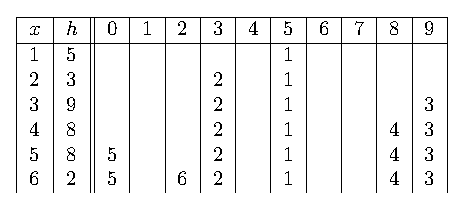
\includegraphics{linearprobing}
  %\begin{tabular}{|l|c||m{0.35cm}|p{0.35cm}|p{0.35cm}|p{0.35cm}|p{0.35cm}|p{0.35cm}|p{0.35cm}|p{0.35cm}|p{0.35cm}|p{0.35cm}|}\hline
  \begin{tabular}{|c|c|| *{10}{>{\centering\arraybackslash}p{0.35cm}|} } \hline
    $\#$ & $h(x)$ & $0$ & $1$ & $2$ & $3$ & $4$ & $5$ & $6$ & $7$ & $8$ & $9$ \\ \hline
    1 & $5$ & & & & & & $x_1$ & & & &\\
    2 & $3$ & & & & $x_2$ & & -- & & & &\\
    3 & $9$ & & & & -- & & -- & & & & $x_3$ \\
    4 & $8$ & & & & -- & & -- & & & $x_4$ & -- \\
    5 & $8$ & $x_5$ & & & -- & & -- & & & -- & -- \\
    6 & $2$ & -- & & $x_6$ & -- & & -- & & & -- & -- \\ \hline
  \end{tabular}
  \caption{A linear probing hash table undergoing the sequential
    insertion of elements $x_1, \ldots, x_6$. In the end, we see that
    $x_2$ and $x_6$ are in a block of size $2$; $x_1$ in a block of
    its own; and $x_3, x_4, x_5$ are in a block of size $3$.}
  \figlabel{linearprobing}
\end{figure}


\begin{lem}\lemlabel{linear-probing-lemma}
  Fix some $x \in \Omega$. In a linear probing hash table with
  $c > e$, the probability that $x$ belongs to a block of size at
  least $t$ satisfying
  \[
  t \log (c/e) - \log t \geq s + O(1)
  \]
  is at most $2^{-s}$.
\end{lem}
\begin{proof}
  Again, we encode the sequence $h(\Omega) = (h(x_1), \ldots, h(x_n))$
  which, for the same reason, is uniformly chosen from a set of size
  $m^n$.

  Suppose that $x$ belongs to a block of size $t$. Our encoding begins
  by providing the first index $i$ of the block containing $x$; then
  the set of the remaining $t - 1$ values in the block, which we call
  $y_1, \ldots, y_{t - 1}$; followed by enough information to decode
  the hash values $h(x), h(y_1), \ldots, h(y_{t-1})$; and finally, the
  hash values of the $n - t$ remaining elements of $\Omega$.

  Note that each of the values $h(x) - i, h(y_1) - i, \ldots,
  h(y_{t-1}) - i$ are within the range $0, 1, \ldots, t - 1$ modulo
  $m$, and so the hash values $h(x), h(y_1), \ldots, h(y_{t-1})$ can
  be encoded using $\lceil t \log t \rceil$ bits. From this
  discussion, we see that our code uses at most
  \begin{align*}
    |C(h(\Omega))| &\leq \log n + \log \binom{n}{t - 1} + t \log t + (n - t) \log m + O(1) \\
                   &\leq \log m^n + t\log n + (t - 1)\log e + \log t - t \log m + O(1) \tag{by \eqref{binom-code-loose}}\\
                   &\leq \log m^n + t\log (e/c) + \log t + O(1) \\
                   &\leq \log m^n - s
  \end{align*}
  bits, as long as $t$ is such that
  \[
  t \log (c/e) - \log t \geq s + O(1).
  \]
  The result follows from \lemref{uel}.
\end{proof}

%\begin{thm}\thmlabel{linear-probing-search}
%  Any operation in a linear probing hash table with $c > e$ takes time
%  at most $2 \log n + O(1)$ with probability $1 - O(1/n)$.
%\end{thm}
%\begin{proof}
%  Choose $s = 2 \log n$ in the previous lemma, so that any fixed $x
%  \in \Omega$ is contained in a block of size $2 \log n + O(1)$ with
%  probability $O(1/n^2)$. Then, by the union bound, no element is
%  contained in a block of size $2 \log n + O(1)$ with probability $1 -
%  O(1/n)$.
%  %A similar argument gives $O(1)$ expected time for any operation.
%\end{proof}

\begin{thm}
  A linear probing hash table with $c > e$ achieves $O(1)$ expected
  time for all operations.
\end{thm}
\begin{proof}
  Let $S$ denote the size of the largest block in such a hash
  table. From \lemref{linear-probing-lemma}, any fixed $x \in \Omega$
  is contained in a block of size at least $2s/\log (c/e) + d$ with
  probability at most $2^{-s}$, for some constant $d$. Then,
  \begin{align*}
    \E[S] &= \sum_{s = 1}^\infty \Pr[S \geq s] = \sum_{s = 1}^{d} \Pr[S \geq s] + \sum_{s = 1}^\infty \Pr[S \geq s + d] \\
          &\leq d + \sum_{s = 1}^\infty 2^{-s \log (c/e)/2} = d + \sum_{i = 1}^\infty \left(\frac{c}{e}\right)^{-s/2} = O(1). \qedhere
  \end{align*}
\end{proof}

%\subsection{Double Hashing}
%
%Encode the string $h_1(x_1) h_2(x_1) \ldots h_1(x_n)
%h_2(x_n)$. Suppose that some $x$ is contained in a block of size $t$.
%
%We encode $R$ by providing the first index $i$ of the block containing
%$x$; then the set of the remaining $t - 1$ values in the block which
%we call $y_1, \ldots, y_{t - 1}$; followed by enough information to
%decode the hash values $h(x), h(y_1), \ldots, h(y_{t-1})$; and
%finally, the hash values of the $n - t$ remaining elements of $X$.

\subsection{Cuckoo Hashing}\seclabel{cuckoo-hashing}

Cuckoo hashing is a simple and efficient hashing solution developed by
Pagh and Rodler which achieves $O(1)$ deterministic search
time~\cite{pagh.rodler:cuckoo}. The encoding arguments in this
section, due to P\u{a}tra\c{s}cu~\cite{patrascu:cuckoo}, neatly
establish some of the nice properties of cuckoo hashing.

The hash table consists of two arrays $A$ and $B$ of size $m = 2n$,
and two hash functions $h, g : \Omega \to \{1, \ldots, m\}$. To insert
an element $x$ into the hash table, we insert it into $A[h(x)]$; if
$A[h(x)]$ already contains an element $y$, we insert $y$ into
$B[g(y)]$; if $B[g(y)]$ already contains some element $z$, we insert
$z$ into $A[h(z)]$, etc. If an empty location is eventually found, the
algorithm terminates successfully. If a cycle is detected, then the
hash table is rebuilt using different hash functions. Any element $x$
either is held in $A[h(x)]$ or $B[g(x)]$, so we can search for $x$ in
$O(1)$ time.

To study the performance of insertion in cuckoo hashing, we study the
random bipartite \emph{cuckoo graph} $G$, where $V(G) = A \cup B$ with
bipartition $(A, B)$, with each vertex corresponding either to a
location in the array $A$ or $B$, and with edge multiset
$E(G) = \{(h(x), g(x)) : x \in \Omega\}$. Note that in this graph,
each edge corresponds to an element of $x$, and each vertex
corresponds to a position in the hash table.

An edge-simple path is a path which uses each edge at most once. Such
a path in this graph describes the potential motion of keys in a hash
table insertion. Thus, in bounding the length of edge-simple paths in
the cuckoo graph, we bound the worst case insertion time.
\begin{lem}\lemlabel{cuckoo-path-length}
  The cuckoo graph has an edge-simple path of length greater than
  $s + \log n + O(1)$ with probability at most $2^{-s}$.
\end{lem}
\begin{proof}
  We encode $G$ by presenting its set of edges. Since each endpoint of
  an edge is chosen independently and uniformly at random from a set
  of $n$ choices, then the set of all edges is chosen uniformly from a
  set of size $m^{2n}$.

  Suppose that some vertex $v$ is the endpoint of an edge-simple path
  of length $t$; such a path has $t + 1$ vertices and $t$ edges. In
  the encoding, we present the $t$ edges of the path in order; then,
  we indicate whether $v \in A$ or $v \in B$; and we give the $t + 1$
  vertices in order starting from $v$; and finally, the remaining
  $2n - 2t$ endpoints of edges of the graph. This code has length
  \begin{align*}
    |C(G)| &\leq t \log n + 1 + (t + 1) \log m + (2n - 2t) \log m + O(1)\\
           &= \log m^{2n} + t \log n - t \log m + \log m + O(1) \\
           &= \log m^{2n} - t + \log n + O(1) \tag{since $m = 2n$} \\
           &\leq \log m^{2n} - s
  \end{align*}
  for $t \geq s + \log n + O(1)$. We finish by applying \lemref{uel}.
\end{proof}

Choosing $s = \log n$ and applying the union bound, we see that
successful insertion takes time at most $2 \log n + O(1)$ with
probability $1 - O(1/n)$.

The cuckoo hashing insertion algorithm can fail if some subgraph of
the cuckoo graph contains more edges than vertices, since edges
correspond to keys, and vertices correspond to array locations.
\begin{lem}\lemlabel{cuckoo-failure}
  Fix some vertex $v \in A$. The probability that $v$ is part of a
  subgraph with more edges than vertices is $O(1/n^2)$.
\end{lem}
\begin{proof}
  Suppose that $v$ is part of a subgraph with more edges than
  vertices, and in particular a minimal such subgraph with $t + 1$
  edges and $t$ vertices. Such a subgraph appears exactly as in
  \figref{cuckoo-cycles}. For every such subgraph, there are two edges
  $e_1$ and $e_2$ whose removal disconnects the graph into two paths
  of length $t_1$ and $t_2$ starting from $v$, where
  $t_1 + t_2 = t - 1$.

  \begin{figure}
    \centering
    \begin{subfigure}[b]{0.3\textwidth}
      \includegraphics{cuckoo1}
      \caption{A cycle with a chord.}
    \end{subfigure}
    \quad\quad
    \begin{subfigure}[b]{0.6\textwidth}
      \includegraphics{cuckoo2}
      \caption{Two cycles connected by a path.}
    \end{subfigure}
    \caption{The potential minimal subgraphs of the cuckoo graph.}
    \figlabel{cuckoo-cycles}
  \end{figure}

  We encode $G$ by presenting Elias $\delta$-codes for the values of
  $t_1$ and $t_2$; then the edges of the above paths in order; then
  the vertices of the paths in order; and the edges $e_1$ and $e_2$;
  and finally the remaining $2n - 2(t + 1)$ endpoints of edges in the
  graph. Such a code has length
  \begin{align*}
    |C(G)| &\leq (t - 1)(\log n + \log m) + 2\log n + (2n - 2(t + 1))\log m + O(\log t) \\
           &= \log m^{2n} - 2\log m - t + O(\log t) \\
           &\leq \log m^{2n} - 2\log n + O(1).
  \end{align*}
  We finish by applying \lemref{uel}.
\end{proof}

From the union bound, we obtain the following:
\begin{cor}
  Cuckoo hashing succeeds upon insertion of $n$ elements with
  probability $1 - O(1/n)$.
\end{cor}

%\begin{rem}
%  TALK ABOUT HAVING MORE ARRAYS AND LOAD FACTOR AND SHIT LIKE THAT.
%\end{rem}

%Hashing analyzed through random bipartite
%graphs. \cite{pagh.rodler:cuckoo} \cite{patrascu:cuckoo}

\subsection{2-Choice Hashing}

We showed in \secref{balls-in-urns} that if $n$ balls are thrown
independently and uniformly at random into $n$ urns, then the maximum
number of balls in any urn is $O(\log n/\log \log n)$ with high
probability. In 2-choice hashing, another instance of hashing with
chaining, each ball is instead given a choice of two urns, and the urn
containing the fewer balls is preferred.

More specifically, we are given two hash functions $h, g : \Omega \to
\{1, \ldots, m\}$. Each value of $h$ and $g$ points to one of $m$
lists. The element $x \in \Omega$ is appended to the smaller list
between $h(x)$ and $g(x)$ during an insertion. The worst case search
time is at most the maximum number of hashing collisions, or the
length of the longest list.

Perhaps surprisingly, the simple change of having two choices instead
of only one results in an exponential improvement over the strategy of
\secref{balls-in-urns}. Indeed, 2-choice hashing was first studied by
Azar \emph{et al.}~\cite{azar:multiplechoice}, who showed that the
expected maximum size of an urn is $\log \log n + O(1)$. Our encoding
argument is based on V\"{o}cking's use of witness trees to analyze
2-choice hashing~\cite{vocking:witness}.

As in \secref{cuckoo-hashing}, we use random graphs to study the
performance of 2-choice hashing. Let $G$ be the random multigraph with
$V(G) = \{1, \ldots, m\}$, where $m = cn$ for some constant $c > e$,
and $E(G) = \{(h(x), g(x)) : x \in \Omega\}$.

%\begin{lem}
%  The multigraph $G$ has an edge-simple path of length greater than
%  $s + \log n + O(1)$ with probability at most $2^{-s}$.
%\end{lem}
%\begin{proof}
%  The proof is similar to that of \lemref{cuckoo-path-length}: again,
%  we encode the set of edges.
%
%  Suppose some vertex $v$ is the endpoint of an edge-simple path of
%  length $t$. We encode this path by presenting the $t$ edges in
%  order, including their orientation; then, the $t + 1$ vertices,
%  starting from $v$; and finally, the remaining $2n - 2t$ endpoints of
%  edges in the graph. Our code has length
%  \begin{align*}
%    |C(G)| &\leq t\log 2n + (t + 1)\log m + (2n - 2t)\log m + O(1) \\
%           &= 2n \log m + t \log 2n - t \log m + \log m + O(1) \\
%           &= \log m^{2n} + t \log \frac{2n}{m} + \log m + O(1) \\
%           &\leq \log m^{2n} + \log n - t + O(1) \\
%           &\leq \log m^{2n} - s,
%  \end{align*}
%  as long as $t \geq s + \log n + O(1)$, so apply \lemref{uel}.
%\end{proof}

\begin{lem}\lemlabel{two-choice-two-cycles}
  $G$ has a subgraph with more edges than vertices with probability
  $O(1/n)$.
\end{lem}
\begin{proof}
  The proof is similar to that of \lemref{cuckoo-failure}, with an
  additional application of the union bound. More specifically, we can
  encode $G$ by giving the same encoding as in
  \lemref{cuckoo-failure}, with an additional bit for each edge
  $(u, v)$ in the encoding, indicating whether $u = h(x)$ and
  $v = g(x)$, or $u = g(x)$ and $v = h(x)$. Our code thus has length
  \begin{align*}
    |C(G)| &\le (t - 1)(\log n + \log m) + 2 \log n + (2n - 2(t + 1))\log m + t + O(\log t) \\
           &= \log m^{2n} - 2 \log n - t \log c + t + O(\log t) \\
           &\le \log m^{2n} - 2 \log n + O(1) ,
  \end{align*}
  since $\log c > 1$.
\end{proof}


%\begin{lem}\lemlabel{two-choice-two-cycles}
%  With probability $1 - O(1/n)$, $G$ has no subgraph with more edges
%  than vertices.
%\end{lem}
%\begin{proof}
%  Again, the proof is similar to that of \lemref{cuckoo-failure}, with
%  an additional application of the union bound.
%\end{proof}

%\begin{lem}
%  Fix some $v \in \{1, \ldots, m\}$. The probability that $v$ belongs
%  to a component of $G$ of size at least $2 \log n$ is $O(1/n^2)$.
%\end{lem}
%\begin{proof}
%  Suppose $G$ has a connected component $C$ containing $v$ with
%  $t - 1$ edges and at most $t$ vertices. We encode the edge set of
%  $G$ by providing the set of vertices in a spanning tree of $C$
%  rooted at $v$; then the shape of this tree; and the labels of the
%  $t - 1$ edges encountered in an inorder traversal of this tree; and
%  finally the remaining $2(n - t + 1)$ endpoints of edges. By Cayley's
%  formula and since $G$ is a multigraph, there are at most $t^{t - 2}$
%  spanning trees of $G$ rooted at $v$. In total, our code has length
%  \begin{align*}
%    |C(G)| &\leq \log {m \choose t - 1} + (t - 2) \log t + (t - 1) \log n + 2 (n - t + 1) \log m + O(1) \\
%           &\leq 2n \log m - (t - 1) \log (c/e) - \log t + O(1) & \text{(by \eqref{binom-code-loose})} \\
%           &\leq \log m^{2n} - s,
%  \end{align*}
%  as long as $t$ is such that
%  \[t \log (c/e) + \log t \geq s + O(1).\]
%  In particular, if we choose $s = 2 \log n$, applying \lemref{uel}
%  tells us that $C$ has size at least $2 \log n$ with probability
%  $O(1/n^2)$.
%\end{proof}
%
%\begin{cor}\corlabel{two-choice-component-size}
%  With probability $1 - O(1/n)$, every component of $G$ has size at
%  most $2 \log n$.
%\end{cor}

\begin{lem}\lemlabel{two-choice-component-size}
  $G$ has a component of size at least $(2/\log(c/e))\log n + O(1)$
  with probability $O(1/n)$.
\end{lem}
\begin{proof}
  Suppose $G$ has a connected component $X$ with $t - 1$ edges and at
  most $t$ vertices. We encode the edge set of $G$ by providing the
  set of vertices in a spanning tree of $X$, and we choose to root
  this tree at the first vertex described in this set; then the shape
  of this tree; and the labels of the $t - 1$ edges encountered in an
  inorder traversal of this tree; and finally the remaining
  $2(n - t + 1)$ endpoints of edges. By Cayley's formula and since $G$
  is a multigraph, there are at most $t^{t - 2}$ rooted spanning trees
  of $G$. In total, our code has length
  \begin{align*}
    |C(G)| &\le \log \binom{m}{t} + (t - 2) \log t + (t - 1) \log n + 2 (n - t + 1) \log m + O(1) \\
           %&\le 2n \log m + t\log m + t\log e - 2\log t + (t-1)\log n - 2(t-1)\log m \tag{by \eqref{binom-code-loose}} \\
           &\le \log m^{2n} - t\log c + t\log e - 2\log t + \log n + O(1) \tag{by \eqref{binom-code-loose}} \\
           &\le \log m^{2n} - s ,
  \end{align*}
  as long as $t$ is such that
  \[t \log (c/e) + 2\log t \geq s + \log n + O(1) .\]
  In particular, if we choose $s = \log n$, applying \lemref{uel}
  tells us that $X$ has size at least $(2/\log (c/e))\log n + O(1)$
  with probability $O(1/n)$.
\end{proof}

Suppose that when $x$ is inserted, it is placed in a list with $t$
other elements. Then, we say that the age of $x$ is $a(x) = t$.
\begin{thm}
  The cost of any operation in 2-choice hashing is at most
  $\log \log n + O(1)$ with probability $1 - O(1/n)$.
\end{thm}
\begin{proof}
  Suppose that some element $x$ has $a(x) = t$. This leads to a binary
  \emph{witness tree} $T$ of height $t$ as follows.

  The root of $T$ is the element $x$. When $x$ was inserted into the
  hash table, it had to choose between the lists $h(x)$ and $g(x)$,
  both of which contained at least $t - 1$ elements; in particular,
  $h(x)$ has an element $x_h$ with $a(x_h) = t - 1$, and $g(x)$ has an
  element $x_g$ with $a(x_g) = t - 1$. The elements $x_h$ and $x_g$
  become left and right children of $x$ in $T$. The process continues
  recursively. If some element appears more than once on a level, we
  only recurse on its leftmost occurence.

  Note that each vertex of $T$ corresponds to the edge $(h(x), g(x))$
  of $G$. Moreover, the subgraph of $G$ induced by the edges
  $\{(h(x), g(x)) : x \in V(T)\}$ is connected.

  Suppose that some node appears more than once on a level of
  $T$. From above, this means that some component of $G$ has a
  cycle. If this happens twice, then $G$ has a subgraph with more
  edges than vertices. By \lemref{two-choice-two-cycles}, this happens
  with probability $O(1/n)$. If instead this happens at most once,
  then $T$ has at most one subtree removed, so $T$ has at least $2^t$
  nodes. If we choose $t = \ceil{\log \log n + d}$, then $T$ has at
  least $2^d \log n$ nodes, which we know from
  \lemref{two-choice-component-size} happens with probability $O(1/n)$
  for a sufficiently large choice of the constant $d$.
\end{proof}

%\subsection{Robin-Hood Hashing}
%Use random hypergraphs to encode the sequence:
%\begin{align*}
%  & h_1(x_1) \ldots h_k(x_1) \\
%  & h_1(x_2) \ldots h_k(x_2) \\
%  & \ldots \\
%  & h_1(x_n) \ldots h_k(x_n)
%\end{align*}

%Suppose that some element $x$ has $a(x) = t$. Then, this leads to a
%witness tree $T$ of height $t$ as follows.

%The root of $T$ is $x$. Let $x_1, \ldots, x_{t - 1}$ denote the
%sequence of elements currently held in
%$A[h_1(x)], \ldots, A[h_{t-1}(x)]$. When $x$ was moved from position
%$h_i(x)$, it competed with an older element $x_i'$ with
%$a(x_i') \geq i$, so $a(x_i) \geq a(x_i') \geq i$. Let $x$ have
%children $x_1, \ldots, x_{t - 1}$ in sequence, and recurse on them. If
%an element appears more than once, only recurse on its first
%occurence.

%Let $H = (V, E)$ be the hypergraph with vertices $\{1,\ldots, m\}$,
%and hyperedges $\{(h_1(x), \ldots, h_k(x)) : x \in X\}$. Each vertex
%of $T$ corresponds to a hyperedge in $H$, and the subhypergraph of $H$
%induced by these hyperedges is connected.

%\begin{thm}[Lavault]
%  The number of $k$-uniform hypertrees with $n$ edges is:
%  \[\frac{(n(k - 1))!}{n! (k - 1)!} (n(k - 1) - 1)^n\]
%\end{thm}

%Ahem... look at the bipartite incidence graph with bipartition
%$(V, E)$, such that $v \sim e$ if $h_i(v) \in e$ for some $i$.

%If some element $x \in X$ has $a(x) = t$, then

%--

%Consider the graph on vertex set $X^k$, with edges
%$(h_1(x), h_2(x)), (h_2(x), h_3(x)), \ldots, (h_{k-1}(x), h_k(x))$ for
%every $x \in X$. If there exists an $x \in X$ with $a(x) = t$, then
%the above witness tree gives a large connected component of the graph.
%\begin{align*}
%  \log {km \choose t - 1} + (t - 2)\log t 
%\end{align*}

\section{Bipartite Expanders}

Expanders are families of graphs which share some isoperimetric
quality, \emph{i.e.}~where subgraphs ``expand'' in their
neighbourhoods. These graphs have received much research attention,
and have been shown to have many applications in computer
science. See, for instance, the survey by Hoory, Linial, and
Wigderson~\cite{hoory.linial.ea:expander}.

Though expanders have proven to have fascinating qualities and be
remarkably useful, they have yet been difficult to construct. The
first proof of existence of expanders by Pinkser was
probabilistic~\cite{pinsker:on}. The first explicit construction,
given by Margulis, relied on advanced concepts in representation
theory~\cite{margulis:explicit}. Later constructions have become
simpler to analyze.

We offer an encoding argument to prove that a random bipartite graph
is an expander with high probability. Indeed, expanders are often
called ``pseudorandom'' graphs due to their many shared properties
with random graphs; one should expect, just as a random graph is
incompressible, so too are expanders.

There are many different notions of expansion. We will consider what
is commonly known as vertex expansion in bipartite graphs.
\begin{defn}
  Fix some $0 < \alpha \leq 1$. A bipartite graph $G$ with bipartition
  $(A, B)$ is a \emph{$(c, \alpha)$-expander} if
  \begin{align*}
    \min_{\substack{{A' \subseteq A}\\{|A'| \leq \alpha |A|}}} \frac{|N(A')|}{|A'|} \geq c,
  \end{align*}
  where $N(A') \subseteq B$ is the set of neighbours of $A'$ in $G$.
\end{defn}

Let $G$ be a random bipartite graph with bipartition $(A, B)$ where
$|A| = |B| = n$ and such that each vertex in $A$ is connected to three
vertices chosen uniformly at random in $B$.

\begin{thm}
  For some constant $\alpha > 0$, $G$ is a $(3/2, \alpha)$-expander
  with probability at least $1 - O(n^{-1/2})$.
\end{thm}
\begin{proof}
  Suppose that $G$ is not a $(3/2, \alpha)$-expander, so there exists
  some $A' \subseteq A$ where $|A'| \leq \alpha |A|$ and
  \[\frac{|N(A')|}{|A'|} < 3/2.\]
  We encode the graph $G$ by encoding its edge set, which is chosen
  uniformly at random from a set of size $n^{3n}$.

  Our encoding presents the value $k = |A'|$ using an Elias
  $\gamma$-code; then the sets $A'$ and $N(A')$, and the edges between
  them; and finally, the remaining edges of the graph. This costs
  \begin{align*}
    |C(G)| &\leq 2\log k + \log {n \choose k} + \log {n \choose 3k/2} + 3k \log (3k/2) + (3n - 3k)\log n + O(1) \nonumber\\
           &\leq \log n^{3n} - (k/2)\log n + (k/2)\log k + \beta k + 2 \log k + O(1) \tag{by \eqref{binom-code-loose}}\\
           &= \log n^{3n} - s(k) \nonumber
  \end{align*}
  bits, where $\beta = (3/2) \log (3/2) + (5/2) \log e$. Note that
  \[
  \frac{d^2}{d k^2} s(k) = \frac{4 - k}{2k^2} \log e ,
  \]
  so $s(k)$ is concave for all $k \geq 4$. Thus, $s(k)$ is minimized
  either when $k = 1, 2, 3, 4,$ or $k = \alpha n$. We have
  \begin{align*}
    s(1) &= (1/2)\log n + c_1, &  s(2) &= \log n + c_2, \\
    s(3) &= (3/2) \log n + c_3, & s(4) &= 2 \log n + c_4,
  \end{align*}
  for constants $c_1, c_2, c_3, c_4$. For $k=\alpha n$ we have
  \[
  s(\alpha n) = (\alpha n/2)\log \left(\frac{1}{2^{2 \beta}
      \alpha}\right) - 2 \log \alpha n + O(1)
  \]
  and $2^{-s(\alpha n)} = 2^{-\Omega(n)}$ for $\alpha < (1/2)^{2
    \beta}$. In each case, apply \lemref{uel}.
\end{proof}

\chapter{Non-Uniform Encoding and Applications}\chlabel{nuel}
The partial prefix-free codes designed and studied in this chapter
will all be denoted $C : \Omega \to \{0, 1\}^* \cup \{\bot\}$, where
$\Omega$ is to be understood from context.

\section{The Non-Uniform Encoding Lemma}

We can extend \lemref{uel} to handle non-uniform input distributions
with a result of Barron, and independently rediscovered through a
joint effort between Devroye, Lugosi, and
Morin~\cite{devroye:workshop}. First, recall the following classic
result.

\begin{thm}[Markov's Inequality]\thmlabel{markov}
  For a non-negative random variable $X$ with finite expectation, and
  any $a > 0$,
  \[
  \Pr[X \geq a] \leq \E[X]/a .
  \]
\end{thm}

\begin{lem}[Barron~\cite{barron:dissertation}]\lemlabel{nuel}
  Let $C : \Omega \to \{0, 1\}^* \cup \{\bot\}$ be a partial
  prefix-free code. Let $x \in \Omega$ be chosen with probability
  $p_x$. Then, for any $s \geq 0$,
  \[\Pr\left[\,|C(x)| \leq \log (1/p_x) - s\,\right]
  \leq 2^{-s}.\]
\end{lem}
\begin{proof}
  We see that
  \begin{align}
    \Pr\left[\,|C(x)| \leq \log(1/p_x) - s\,\right] & = \Pr\left[\,\log(1/p_x) - |C(x)| \geq s\,\right] \notag \\
    & = \Pr\left[2^{\log(1/p_x) - |C(x)|} \geq 2^s\right] \notag \\
    & \leq 2^{-s} \E\left[2^{\log(1/p_x) - |C(x)|}\right] \eqlabel{non-uniform-part}
  \end{align}
  by Markov's inequality. Further, by definition of the expected
  value, \eqref{non-uniform-part} becomes
  \begin{align*}
    2^{-s} \E\left[\,2^{\log(1/p_x) - |C(x)|}\,\right] = 2^{-s} \left(\sum_{C(x) \neq \bot} p_x 2^{\log(1/p_x) - |C(x)|}\right) = 2^{-s} \left(\sum_{C(x) \neq \bot} 2^{-|C(x)|} \right).
  \end{align*}
  By \lemref{kraft-inequality},
  $\sum_{C(x) \neq \bot} 2^{-|C(x)|} \leq 1$, and the result is
  obtained.
\end{proof}

Indeed, this non-uniform encoding lemma immediately implies
\lemref{uel} by choosing $p_x = 1/|\Omega|$.

\begin{prop}\proplabel{non-uniform-binary-runs-loose}
  Let $x_1, \ldots, x_n$ be independent $\text{Bernoulli}(p)$ random
  variables. Then, the probability that $x = x_1 \cdots x_n \in \{0,
  1\}^n$ has a run of ones of length at least
  \[\frac{s + \ceil{\log n} + 1}{\log (1/p)}\]
  is at most $2^{-s}$.
\end{prop}
\begin{proof}
  The proof is almost identical to that of
  \propref{binary-runs}. Suppose that $x$ has a run of ones of length
  $t \geq (s + \ceil{\log n} + 1)/\log (1/p)$.

  Our code begins with the index where this run begins, which allows
  us to deduce $t$ one bits of $x$; and then the Shannon-Fano code
  with parameter $p$ for the remaining bits. Recall that $n_1(x)$ and
  $n_0(x)$ denote the number of one and zero bits in $x$,
  respectively. In total, this code has length
  \begin{align*}
    |C(x)| &= \ceil{\log n} + \left\lceil (n_1(x) - t) \log \frac{1}{p} + n_0(x) \log \frac{1}{1 - p} \right\rceil \\
           &\leq \log \frac{1}{p_x} + \ceil{\log n} - t \log \frac{1}{p} + 1 \\
           &\leq \log \frac{1}{p_x} - s
  \end{align*}
  by our choice of $t$, and since $p_x = p^{n_1(x)} (1 -
  p)^{n_0(x)}$. The result follows from \lemref{nuel}.
\end{proof}

This result appears even more unnatural than that of
\propref{binary-runs}---again, we can prove that this bit string has a
run of length at least $(s + \log n)/\log (1/p)$ by appealing directly
to probability. We will show how this can be resolved in \chref{el}.

\section{The Erd\H{o}s-R\'{e}nyi Random Graph}

\begin{defn}
  The \emph{Erd\H{o}s-R\'{e}nyi random graph} $G_{n, p}$ is the space
  of random undirected graphs on $n$ vertices in which each edge is
  included independently at random with probability $p$.
\end{defn}

The study of the Erd\H{o}s-R\'{e}nyi random graph model played an
important role in the popularization of the now pervasive
probabilistic method~\cite{alon:probabilistic, erdos:randomgraphs}. In
general, probabilistic proofs appear to be easily adapted into
encoding arguments. We show how it is simple to recover some of
Erd\H{o}s and R\'{e}nyi's classic results about $G_{n, p}$.

\begin{lem}\lemlabel{erdos-renyi-lemma}
  The probability that $G \in G_{n, p}$ has a partition $(U, W)$ of
  its vertex set such that $|U| = k$ and there is no edge of $G$ with
  one endpoint in $U$ and the other in $W$ is at most
  $O\left({n \choose k} (1 - p)^{k (n - k)}\right)$.
\end{lem}
\begin{proof}
  We encode $G$ by giving its adjacency matrix $A$, which determines
  the graph. The entire matrix is determined by its portion which lies
  above its diagonal, which is a random bit string of length
  $\binom{n}{2}$ in which each bit appears with probability $p$.

  We give a list of the $k$ vertices in $U$, which determines
  $k(n - k)$ non-edges of the graph between $U$ and $W$; and a
  Shannon-Fano code with parameter $p$ for the remaining
  $\binom{n}{2} - k(n - k)$ edges of the graph. This code has length
  \begin{align*}
    |C(G)| &\leq \log {n \choose k} + n_1(A) \log \frac{1}{p} + (n_0(A) - k(n - k)) \log \frac{1}{1 - p} + O(1) \\
           &= \log \frac{1}{p_G} + \log {n \choose k} - k(n - k) \log \frac{1}{1 - p} + O(1) \\
           &= \log \frac{1}{p_G} + \log \left(O\left({n \choose k} (1 - p)^{k(n - k)}\right)\right).
  \end{align*}
  We finish by applying \lemref{nuel}.
\end{proof}

The typical proof of the above result, given by the probabilistic
method, says that this probability is at most
$\binom{n}{k} (1 - p)^{k (n - k)}$. Nevertheless,
\lemref{erdos-renyi-lemma} is sufficient to obtain the classic
threshold connectivity results for the Erd\H{o}s-R\'{e}nyi random
graph.

%As a first application of \lemref{erdos-renyi-lemma}, we establish
%connectivity properties of $G_{n, p}$:
%
\begin{thm}
  When $p = (1 + \eps) \frac{\ln n}{n}$, $G \in G_{n, p}$ has no
  isolated vertices with high probability.
\end{thm}
\begin{proof}
  Choose $k = 1$ in \lemref{erdos-renyi-lemma}. Then, the probability
  that $G$ has an isolated vertex is at most
  \[
  O\left(n \left(1 - (1 + \eps) \frac{\ln n}{n}\right)^{n - 1}\right) =  O\left(n e^{-(1 + \eps) \ln n} (1 + o(1))\right) = O(n^{-\eps}). \hfill \qedhere
  \]
\end{proof}
%We can apply \lemref{erdos-renyi-lemma} and the union bound to show
%that $G$ is connected with high probability.

\begin{thm}
  When $p = (1 + \eps) \frac{\ln n}{n}$, $G \in G_{n, p}$ is
  connected with high probability.
\end{thm}
\begin{proof}
  This follows from \lemref{erdos-renyi-lemma} and the union bound.
\end{proof}
%\begin{proof}
%  By the union bound, the probability that $G$ is disconnected is at
%  most:
%  \begin{align*}
%    \sum_{k = 1}^{n/2} O({n \choose k} (1 - p)^{k(n - k)}) & \leq O(1)\sum_{k = 1}^n {n \choose k} ((1 - p)^{n/2})^k \\
%    & = O(1)[((1 - p)^{n/2} + 1)^n - 1]
%  \end{align*}
%
%  Moreover, since $1 + x \leq e^x$ for all $x \in \R$, we see that
%  \begin{align*}
%    ((1 - p)^{n/2} + 1)^n - 1 & \leq (e^{-pn/2} + 1)^n - 1 \leq e^{e^{-pn^2/2}} - 1 \\
%                              & \leq e^{n^{-(1 + \eps)n/2}} - 1 \to 0
%  \end{align*}

 % $(1 - 1/n)^n = e^{-1} + O(1/n)$

 % $(1 - 1/(n/\ln n^{1+\eps}))^{n} = (e^{-1} + O(\ln n/n))^{\ln n^{1+\eps}}$

 % $= n^{-(1 + \eps)/2} + O(\ln^2 n/n^{2 + \eps})$
  
  %Since $\left(1 - \frac{1}{n}\right)^n = e^{-1} + O(1/n)$, we see
  %that:
  %\begin{align*}
  %  (1 - p)^{n/2} & = \left(1 - (1 + \eps) \frac{\ln n}{n}\right)^{n/2} = n^{-(1 + \eps)/2} + O\left(\frac{\log^2 n}{n^{(3 + \eps)/2}}\right)
  %\end{align*}

  %If $\lim (1 + f(n)) = 1$, then $\lim (1 + f(n))^n = 1$.

  %$\lim e^{n \ln (1 + f(n))}$

  %It can be shown that this probability tends to $0$.
%\end{proof}

%\begin{thm}
%  When $p = (1 - \eps) \frac{\ln n}{n}$, $G \sim G_{n, p}$ is
%  disconnected with high probability.
%\end{thm}
%\begin{proof}
%  Again, we encode $G$'s adjacency matrix $A$.
%
%  If $G$ is connected, then it has a spanning tree $T$. We encode $G$
%  by providing the shape of $T$, fixing an arbitrary vertex as its
%  root, which informs us of the presence of $n - 1$ edges in $G$; and
%  then a Shannon-Fano code for the remaining edges in the graph. This
%  costs:
%  \begin{align*}
%    b & \leq (n - 2)\log n + (n_1(A) - (n - 1)) \log \frac{1}{p} + n_0(A) \log \frac{1}{1 - p} + 1 \\
%      & = \log \frac{1}{p_A} + (n - 2) \log n + (n - 1) \log p \\
%      & = \log \frac{1}{p_A} - \log n + (n - 1)\log \ln n^{1 - \eps}
%  \end{align*}%

%  bits. By \lemref{nuel}, we obtain that $G$ is connected with
%  probability $O(\ln n/n)$, so $G$ is disconnected with high
%  probability.
%\end{proof}

\begin{thm}\thmlabel{erdos-renyi-component}
  When $p = \frac{1}{\alpha n}$ for $\alpha > e$, the graph
  $G \in G_{n, p}$ has a component of size at least
  \[
  \frac{\log n + s + O(1)}{\log (\alpha/e)}
  \]
  with probability at most $2^{-s}$.
\end{thm}
\begin{proof}
  We again encode the adjacency matrix $A$ of $G$. Suppose that $G$
  has a component of size $t$. We encode $G$ by giving these $t$
  vertices; the shape of a spanning tree for this component; and a
  Shannon-Fano code with parameter $p$ for the remaining edges of the
  graph. This code has length
  \begin{align*}
    |C(G)| &\leq \log \binom{n}{t} + (t - 2) \log t + (n_1(A) - (t - 1))\log \frac{1}{p} + n_0(A) \log \frac{1}{1 - p} + O(1) \\
           &\leq \log \frac{1}{p_G} + t \log n - t \log t + t \log e + t \log t - (t - 1) \log \frac{1}{p} + O(1) \tag{by \eqref{binom-code-loose}} \\
           &\leq \log \frac{1}{p_G} + \log n + t \log e - t \log \alpha + O(1) \\
           &= \log \frac{1}{p_G} + \log n - t \log \frac{\alpha}{e} + O(1) \\
           &\leq \log \frac{1}{p_G} - s
  \end{align*}
  by our choice of $t$. We finish by applying \lemref{nuel}.
\end{proof}
\begin{rem}
  This result and its proof are similar to that of
  \lemref{two-choice-component-size} from our study of random
  multigraphs in 2-choice hashing. Indeed, the random multigraph we
  studied contained exactly $n$ edges for $cn$ vertices,
  \emph{i.e.}~$n/c$ edges for $n$ vertices, and the
  Erd\H{o}s-R\'{e}nyi graph from \thmref{erdos-renyi-component} is
  expected to contain $(n - 1)/(2 \alpha)$ edges for $n$
  vertices. Since the random graph models are so similar, and since
  the edge densities we are concerned with are practically identical,
  this observation should be of no surprise.
\end{rem}

A triangle in a graph is a $K_3$ subgraph. Our nextt encoding argument
bounds the probability that $G_{n, c/n}$ has no triangle. It is easy
to see that the expected number of triangles in $G_{n, c/n}$ is
$\binom{n}{3} (c/n)^3 = c/6 - O(1/n)$, so $G_{c, c/n}$ is expected to
have at least one triangle for large enough values of $c$. However, a
typical proof that $G_{n, c/n}$ has a triangle with non-negligible
probability usually uses the second moment method which involves
computing the variance of the number of
triangles~\cite{souza:notes}. To show that $G_{n, c/n}$ has a triangle
with exponential probability is even more complicated, and a proof of
this result would still typically rely on an advanced probabilistic
inequality~\cite{alon:probabilistic}. Our argument is easy and avoids
this trouble.

We will, however, rely on the following classic result, which we later
prove in \chref{el} using an encoding argument.
\newtheorem*{thm:chernoff}{Theorem 5.7}%{\begin{NoHyper}\thmref{chernoff}\end{NoHyper}}
%\newreptheorem{theorem}{Theorem}
\begin{thm:chernoff}[Additive Chernoff Bound~\cite{mulzer:encoding}]
  Let $B$ be a $\text{Binomial}(n, p)$ random variable. Then
  \[
  \Pr[B \leq (p - t)n] \leq 2^{-n D(p - t \| p)}
  \]
  where
  \[D(p \| q) = p \log \frac{p}{q} + (1 - p) \log \frac{1 - p}{1 -
    q}\]
  is the \emph{Kullback-Leibler divergence} or \emph{relative entropy}
  between Bernoulli random variables with parameters $p$ and $q$.
\end{thm:chernoff}

\begin{figure}
  \centering
  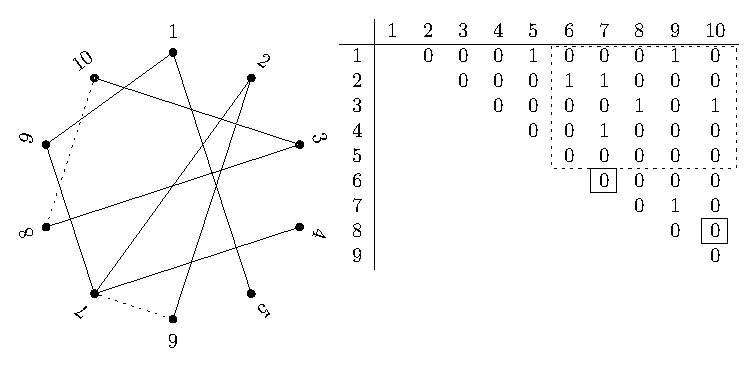
\includegraphics{triangles}
  \caption{The random graph $G_{n, c/n}$ has triangles when $c$ is
    large enough. The depicted zero bits in the adjacency matrix can
    be deduced from the first $n/2$ rows.}
  \figlabel{triangles}
\end{figure}

\begin{thm}\thmlabel{triangles-up}
  When $p = c/n$, the graph $G \in G_{n, p}$ contains at least one
  triangle with probability at least $1 - 2^{-\varOmega(c^3)}$.
\end{thm}
\begin{proof}
  Refer to \figref{triangles}. Suppose that $G$ contains no
  triangles. We encode the adjacency matrix $A$ of $G$. Let $M$ be the
  $n/2 \times n/2$ submatrix of $A$ determined by the rows
  $1, \ldots, n/2$ and the columns $n/2 + 1, \ldots, n$. Note that
  $\E[n_1(M)] = cn/4$.

  Suppose that $n_1(M) < cn/8$. Note that $n_1(M)$ is a
  $\text{Binomial}(n^2/4, c/n)$ random variable whose value deviates
  largely from its mean. Then, by Chernoff's bound, we obtain that
  \begin{align*}
    \Pr[n_1(M) < cn/8] &= \Pr[n_1(M) < (c/2n) (n^2/4)] \leq 2^{-(n^2/4) D(c/2n \| c/n)}.
  \end{align*}
  The function $D(x/2 \| x) : [0, 1] \to \R$ has
  derivative
  \[\frac{d}{dx} D(x/2 \| x) = - \frac{1}{2} + \log \frac{1 - x}{1 -
    x/2} + \frac{\log e}{2(1 - x)}\]
  which is strictly increasing, so
  $D(x/2 \| x) \geq \left(\frac{\log e - 1}{2}\right)x$. Thus,
  $D(c/2n \| c/n) = \varOmega(c/n)$, and
  \[\Pr[n_1(M) < cn/8] \leq 2^{-\varOmega(cn)}.\]

  Suppose instead that $n_1(M) \geq cn/8$. Note that if $A_{i,j} = 1$
  and $A_{i, k} = 1$ for $i < j < k$, then $A_{j, k} = 0$ since $G$
  has no triangles. Let $m_i$ denote the number of ones in the
  $i$\textsuperscript{th} row of $M$. Since the function $x(x - 1)/2$
  is convex, then by \thmref{jensen}, we have that
  \[
  \frac{1}{n/2} \sum_{i = 1}^{n/2} {m_i \choose 2} \geq \binom{2
    n_1(M)/n}{2}.
  \]
  From these observations, we see that by specifying the rows $1,
  \ldots, n/2$ of $A$, we can deduce
  \[m = \sum_{i = 1}^{n/2} {m_i \choose 2} \geq \frac{n}{2} {2 n_1(M)/n
    \choose 2} \geq \frac{n}{2} {c/4 \choose 2} = \varOmega(c^2 n)\]
  zero bits in the rows $n/2 + 1, \ldots, n$.

  We encode $G$ by giving a Shannon-Fano code with parameter $p$ for
  the first $n/2$ rows of $A$; and a Shannon-Fano code with parameter
  $p$ for the rest of $A$, excluding the bits which can be deduced
  from the preceding information. Such a code has length
  \begin{align*}
    |C(G)| &\leq n_1(A) \log \frac{1}{p} + (n_0(A) - m) \log \frac{1}{1 - p} + O(1) \\
           &= \log \frac{1}{p_G} - m \log \frac{1}{1 - p} + O(1) \\
           &\leq \log \frac{1}{p_G} - mp + O(1) \\
           &\leq \log \frac{1}{p_G} - \varOmega(c^3).
  \end{align*}
  Applying \lemref{nuel}, we see that $G$ has no triangles with
  probability at most $2^{- \varOmega(c^3)}$.
\end{proof}

\begin{thm}\thmlabel{triangles-down}
  When $p = \frac{1}{\alpha n}$, $G \in G_{n, p}$ has no triangle
  with probability $1 - O(\alpha^{-3})$.
\end{thm}
\begin{proof}
  Suppose that $G$ contains a triangle. We encode the adjacency matrix
  $A$ of $G$. First, we specify the triangle's vertices; and finish
  with a Shannon-Fano code with parameter $p$ for the remaining
  vertices of the graph. This code has length
  \begin{align*}
    |C(G)| &\leq 3 \log n + (n_1(A) - 3) \log \frac{1}{p} + n_0(A) \log \frac{1}{1 - p} + O(1) \\
           &= \log \frac{1}{p_G} + 3 \log n - 3 \log \frac{1}{p} + O(1) \\
           &= \log \frac{1}{p_G} - 3 \log \alpha + O(1) \\
           &= \log \frac{1}{p_G} - \log O(\alpha^3).
  \end{align*}
  We finish by applying \lemref{nuel}.
\end{proof}

Together, \thmref{triangles-up} and \thmref{triangles-down} establish
that $1/n$ is a threshold function for triangle-freeness.

\section{Percolation on the Torus}

Percolation theory studies the emergence of large components in random
graphs. We give an encoding argument proving that percolation occurs
on the torus when edge survival rate is greater than $2/3$. Our line
of reasoning follows what is known as a \emph{Peierls argument}. For
more precise results, including a general study of percolation theory,
see the book by Grimmett~\cite{grimmett:percolation}.

\begin{defn}
  When $\sqrt{n}$ is an integer, the \emph{$\sqrt{n} \times \sqrt{n}$
    torus grid graph} is defined to be the graph with vertex set
  $\{1, \ldots, \sqrt{n}\}^2$, where $(i, j)$ is adjacent to
  $(k, \ell)$ if
  \begin{itemize}
    \item $|i - k| \equiv 1 \pmod{\sqrt{n}}$ and $|j - \ell| = 0$, or
    \item $|i - k| = 0$ and $|j - \ell| \equiv 1 \pmod{\sqrt{n}}$.
    \end{itemize}
\end{defn}

\begin{thm}
  Let $G$ be the subgraph of the $\sqrt{n} \times \sqrt{n}$ torus grid
  graph in which each edge is chosen with probability $p < 1/3$. Then,
  the probability that $G$ contains a cycle of length at least
  \[\frac{s + \log n + O(1)}{\log (1/(3p))}\]
  is at most $2^{-s}$.
\end{thm}
\begin{proof}
  Let $A$ be the bitstring of length $2n$ encoding the existence of
  edges in $G$. Suppose that $G$ contains a cycle $C'$ of length
  $t \geq (s + \log n + O(1))/\log (1/(3p))$. Encode $A$ by giving a
  single vertex $u$ in $C'$; the sequence of directions that the cycle
  moves along from $u$; and a Shannon-Fano code with parameter $p$ for
  the remaining edges of $G$.

  Note that there are four possibilities for the direction of the
  first step taken by $C'$ from $u$, but only three for each
  subsequent choice. Thus, this sequence can be specified by
  $\lceil 2 + (t - 1) \log 3 \rceil$ bits. The total length of our
  code is then
  \begin{align*}
    |C(G)| &\leq \log n + t \log 3 + (n_1(A) - t) \log \frac{1}{p} +
             n_0(A) \log \frac{1}{1 - p} + O(1) \\
           &= \log \frac{1}{p_G} + \log n - t \log \frac{1}{3p} + O(1) \\
           &\leq \log \frac{1}{p_G} - s
  \end{align*}
  by our choice of $t$. We finish by applying \lemref{nuel}.
\end{proof}

The torus grid graph can be drawn in the obvious way without crossings
on the surface of a torus. This graph drawing gives rise to a dual
graph, in which each vertex corresponds to a face in the primal
drawing, and two vertices are adjacent if and only their primal faces
are incident to the same edge. In this sense, the torus grid graph is
self-dual.

The obvious drawing of the torus grid graph also induces drawings for
any of its subgraphs. Such a subgraph also has a dual, where each
vertex corresponds to a face in the dual torus grid graph, and two
vertices are adjacent if and only if their corresponding faces are
incident to the same edge of the original subgraph.

\begin{thm}
  Let $G$ denote the subgraph of the $\sqrt{n} \times \sqrt{n}$ torus
  grid graph in which each edge is chosen with probability greater
  than $2/3$. Then, $G$ has at most one component of size
  $\omega(\log^2 n)$ with high probability.
\end{thm}
\begin{proof}
  See \figref{peierls} for a visualization of this phenomenon. Suppose
  that $G$ has at least two components of size $\omega(\log^2
  n)$. Then, there is a cycle of faces separating these components
  whose length is $\omega(\log n)$. From the discussion above, such a
  cycle corresponds to a cycle of $\omega(\log n)$ missing edges in
  the dual graph, as in \figref{peierlsrare}. From the previous
  result, we know that this does not happen with high probability.
\end{proof}

\begin{figure}
  \centering
  \begin{subfigure}[t]{0.4\textwidth}
    \includegraphics{torusrare}
    \caption{When $p = 0.33 < 1/3$, long cycles are rare. Dotted lines show
      missing edges in the dual.}
    \figlabel{peierlsrare}
  \end{subfigure}
  \quad\quad
  \begin{subfigure}[t]{0.4\textwidth}
    \includegraphics{torusdense}
    \caption{When $p = 0.67 > 2/3$, there is likely only one large
      component.}
  \end{subfigure}
  \caption{Random subgraphs of the $20 \times 20$ torus grid graph.}
  \figlabel{peierls}
\end{figure}

%
%\subsection{Random Independent Sets on the Hypercube}
%
%Consider the hypercube $Q_d$ with bipartition $(E, O)$. Let $I$ be a
%uniformly random independent set of $Q_d$. Consider the value
%$t = \max\{|I \cap E|, |I \cap O|\}$.
%
%Suppose that $|I_0| \geq 2^d/5$. Then


%\section{SOMETHING ELSE???}

\chapter{Encoding with Kraft's Condition}\chlabel{el}

We have seen how \lemref{uel} and \lemref{nuel} can be used to prove
well-known bounds in intuitive and unexpected manners, within some
constant factor or some lower order term. However, when exactness is
required, it may be that neither suffices, even if
\lemref{incremental-code} is used, due to the discrete integral
constraint on codeword lengths, as shown in
\propref{binary-runs}. Instead, we will use a continuous analogue of
\lemref{nuel} due to Mulzer.

Observe that neither \lemref{uel}, \lemref{nuel}, nor any application
of either of these results in \chref{uel} and \chref{nuel} requires
the specification of any prefix-free code; we know, by construction,
that every such code is prefix-free, but we could also deduce from
\lemref{kraft-inequality} that, since our described codes satisfy
Kraft's condition, a prefix-free code with the same codeword lengths
exists. Instead, codeword lengths satisfying Kraft's condition
suffice. Indeed, we will show how such codeword lengths actually need
not be integers; this refinement will allow us to tighten
\lemref{nuel}, thereby tightening all of the results established
throughout the previous chapters.

Let $[0, \infty]$ denote the set of extended non-negative real
numbers, \emph{i.e.}~the usual open interval $[0, \infty)$, including
the formal symbol $\infty$, satisfying all real arithmetic operations
and all usual extended operations. In particular, we have that
$x + \infty = \infty$ for all $x \in [0, \infty]$ and
$2^{-\infty} = 0$. We will also allow that $1/0 = \infty$.

\begin{lem}[Mulzer~\cite{mulzer:encoding}]\lemlabel{el}
  Let $\ell : \Omega \to [0, \infty]$ satisfy Kraft's condition, and
  let $x \in \Omega$ be chosen with probability $p_x$. Then, for any
  $s \geq 0$,
  \[\Pr\left[\,\ell(x) \leq \log (1/p_x) - s\,\right] \leq 2^{-s}.\]
\end{lem}
\begin{proof}
  The proof is identical to that of \lemref{nuel}.
\end{proof}

The sum of functions $\ell : \Omega \to [0, \infty]$ and $\ell' :
\Omega' \to [0, \infty]$ is the function $\ell + \ell' : \Omega \times
\Omega' \to [0, \infty]$, where $(\ell + \ell') (x, y) = \ell(x) +
\ell'(y)$. Note that for any partial codes $C : \Omega \to \{0, 1\}^*
\cup \{\bot\}, C' : \Omega' \to \{0, 1\}^* \cup \{\bot\}$, any $x \in
\Omega$, and any $y \in \Omega'$,
\[(|C| + |C'|)(x, y) = |C(x)| + |C'(y)| = |(C \cdot C')|(x, y).\]
In other words, the sum of these functions describes the length of
codewords in composed codes.

\begin{lem}\lemlabel{composition-tight}
  If $\ell : \Omega \to [0, \infty]$ and $\ell' : \Omega' \to [0,
  \infty]$ satisfy Kraft's condition, then so does $\ell + \ell'$.
\end{lem}
\begin{proof}
  Kraft's condition still holds:
  \[\sum_{(x, y) \in \Omega \times \Omega'} 2^{-(\ell + \ell')(x, y)} = \sum_{x
    \in \Omega} \sum_{y \in \Omega'} 2^{-\ell(x) - \ell'(y)} = \sum_{x
    \in \Omega} 2^{-\ell(x)} \sum_{y \in \Omega'} 2^{-\ell'(y)} \leq
  1. \qedhere\]
\end{proof}
This is analogous to the fact that the composition of prefix-free
codes is prefix-free. This result renders \lemref{incremental-code}
obsolete, and now nothing is wasted in the composition of codes.

\begin{lem}\lemlabel{fixed-length-tight}
  For any probability density $p : \Omega \to [0, 1]$, the function
  $\ell : \Omega \to [0, \infty]$ with $\ell(x) = \log (1/p_x)$
  satisfies Kraft's condition.
\end{lem}
\begin{proof}
  \[\sum_{x \in \Omega} 2^{-\ell(x)} = \sum_{x \in \Omega} 2^{-\log (1/p_x)} =
  \sum_{x \in \Omega} p_x = 1. \qedhere\]
\end{proof}
This now allows us to refine every instance of a fixed-length code and
every instance of a Shannon-Fano code used while encoding so that,
again, nothing is wasted. Note that these lengths now match Shannon's
lower bound from \thmref{noiseless-coding}.

We now give a tight notion corresponding to Elias $\omega$-codes.
\begin{thm}[Beigel~\cite{beigel:elias}]\thmlabel{elias-tight}
  Fix some $0 < \eps < e - 1$. Let $\ell : \N \to [0, \infty]$ have
  \[\ell(i) = \log i + \log \log i + \cdots + \underbrace{\log \cdots \log}_{\text{$\log^* i$ times}} i -
  (\log \log (e - \eps)) \log^* i + O(1).\]
  %\[\ell(i) = \log i + \log^{(2)} i + \ldots + \log^{(\log^* i)} i -
  %\log \log (e - \eps) \log^* i + O(1).\]
  %\[\ell(i) = \log i + \log^{(2)} i + \ldots + \log^{(\log^* i)} i +
  %\log \left(\frac{1}{1 - \ln 2}\right).\]
  Then, $\ell$ satisfies Kraft's condition.
\end{thm}
\begin{thm}[Beigel~\cite{beigel:elias}]
  The function $\ell : \N \to [0, \infty]$ with
  \[\ell(i) = \log i + \log \log i + \cdots + \underbrace{\log \cdots \log}_{\text{$\log^* i$ times}} i -
  (\log \log e) \log^* i + c\]
  does not satisfy Kraft's condition for any choice of the constant
  $c$.
\end{thm}

Recall how the result of \propref{binary-runs} carried an artifact of
binary encoding. Using our new tools, we can now refine this and
recover the exact result.
\begin{prop}
  A uniformly random bit string $x_1 \cdots x_n$ contains a run of at
  least $\log n + s$ ones with probability at most $2^{-s}$.
\end{prop}
\begin{proof}
  Let $\ell : \{0, 1\}^n \to [0, \infty]$ be such that if $x$ contains
  a run of $t \geq \log n + s$ ones, then $\ell(x) = \log n + n - t$,
  and otherwise $\ell(x) = \infty$. We will show that $\ell$ satisfies
  Kraft's condition.

  Recall that a binary string $x = x_1 \cdots x_n$ is said to contain
  a run of $t$ ones if there exists some
  $i \in \{1, \ldots, n - t + 1\}$ such that
  $x_i = \cdots = x_{i + t - 1} = 1$.

  Let the function $f : \{1, \ldots, n - t + 1\} \to [0, \infty]$ have
  $f(i) = \log n$ for all $i$, and
  $g : \{0, 1\}^{n - t} \to [0, \infty]$ have $g(x) = n - t$ for all
  $x$. Both of these functions satisfy Kraft's condition by
  \lemref{fixed-length-tight}. By \lemref{composition-tight}, so does
  the function
  \begin{align*}
    h = f + g : \{1, \ldots, n - t + 1\} \times \{0, 1\}^{n - t} &\to
    [0, \infty],
  \end{align*}
  where $h(i, x) = \log n + n - t$ for all $i$ and $x$. Crucially,
  each element of the set
  $\{1, \ldots, n - t + 1\} \times \{0, 1\}^{n - t}$ corresponds to an
  $n$-bit binary string containing a run of $t$ ones: the element
  $(i, x) \in \{1, \ldots, n - t + 1\} \times \{0, 1\}^{n - t}$, where
  $x = x_1 \cdots x_{n - t}$, corresponds to the binary string
  \[x_1 \cdots x_{i - 1} \underbrace{1 1 \cdots 1}_{\text{$t$ times}} x_i \cdots x_{n - t}.\]
  Therefore, $\ell$ satisfies Kraft's condition. By our choice of
  $t$, we have that $\ell(x) \leq n - s$ if and only if $x$ contains a
  run of $t$ ones. We finish by applying \lemref{el}.
  %Therefore, we can
  %represent any such string by writing the value $i$ in binary,
  %followed by the bits
  %$x_1, \ldots, x_{i - 1}, x_{i + t}, \ldots, x_n$. This
  %representation uses
  %\[\ceil{\log n} + n - t \leq n - s\]
  %bits, by choice of $t$, and allows us to represent any $n$-bit
  %binary string having a run of $t$ or more ones. Therefore, the
  %number of $n$-bit binary strings with a run of $t$ ones is at most
  %$2^{n - s}$, so the probability that a uniformly random $n$-bit
  %binary string contains a run of $t$ ones is at most
  %$2^{n - s}/2^n = 2^{-s}$, as required.
\end{proof}

It is not hard to see how \lemref{el}, \lemref{composition-tight},
\lemref{fixed-length-tight}, and \thmref{elias-tight} can be used to
reframe and refine every encoding argument presented in \chref{uel}
and \chref{nuel}, just as we did in the proof above.

%Given some set $X$, we will say that a function $w : X \to [0, 1]$ is
%a \emph{weight function}. Moreover, if
%\[\sum_{x \in X} w(x) \leq 1,\]
%then $w$ is called \emph{valid}. We can see the above inequality is a
%continuous analogue of \lemref{kraft-inequality}, where if each
%$\log (1/w(x))$ were an integer, then $w$ would describe a prefix-free
%code. It is not surprising then that valid weight functions carry some
%of the properties of prefix-free codes.

%\begin{lem}[Mulzer \cite{mulzer:encoding}]\lemlabel{cnuel}
%  Let $w : X \to [0, 1]$ be a valid weight function, and let $x \in X$
%  be chosen with probability $p_x$. Then, for any $s \geq 1$,
%  \[\Pr[w(x) \geq p_x s] \leq \frac{1}{s}.\]
%\end{lem}
%\begin{proof}
%  Let $Z = \{x \in X : w(x) \geq p_x s\}$. Then
%  \begin{align*}
%    \Pr[w(x) \geq p_x s] = \sum_{x \in Z} p_x \leq \sum_{x \in Z} p_x \frac{w(x)}{p_x s} \leq \frac{1}{s} \sum_{x \in Z} w(x) \leq \frac{1}{s},
%  \end{align*}
%  since $w(x)/p_x s \geq 1$ for any $x \in Z$, and since $w$ is a
%  valid weight function.
%\end{proof}

%\lemref{nuel} for prefix-free codes follows as an immediate corollary,
%choosing $w(x) = 2^{-|C(x)|}$, which is a valid weight function by
%\lemref{kraft-inequality}.

\section{Chernoff Bound}\seclabel{chernoff}

The following proof is due to Mulzer, and serves as a refinement to an
encoding argument given by Devroye, Lugosi, and Morin, which only used
\lemref{nuel} instead of the tight framework developed in this
chapter, and thus was imprecise.

\begin{thm:chernoff}[Additive Chernoff Bound~\cite{mulzer:encoding}]\thmlabel{chernoff}
  Let $B$ be a $\text{Binomial}(n, p)$ random variable. Then
  \[
  \Pr[B \leq (p - t)n] \leq 2^{-n D(p - t \| p)}
  \]
  where
  \[D(p \| q) = p \log \frac{p}{q} + (1 - p) \log \frac{1 - p}{1 -
    q}\]
  is the \emph{Kullback-Leibler divergence} or \emph{relative entropy}
  between Bernoulli random variables with parameters $p$ and $q$.
\end{thm:chernoff}
\begin{proof}
  By definition, $B = \sum_{i = 1}^n x_i$ for independent
  $\text{Bernoulli}(p)$ random variables $x_1, \ldots, x_n$, so $B =
  n_1(x)$ for $x = x_1 \cdots x_n$. We are interested in encoding the
  string $x \in \{0, 1\}^n$.

  Informally, we encode $x$ using a Shannon-Fano code with parameter
  $p - t$. The result of \lemref{fixed-length-tight} allows us to
  ignore the ceiling in the lengths of these codewords. In other
  words, we are interested in the function
  $\ell : \{0, 1\}^n \to [0, \infty]$ with
  \[
  \ell(x) = n_1(x) \log \frac{1}{p - t} + (n - n_1(x)) \log \frac{1}{1 - p + t} .
  \]
  Now, $x$ occurs with probability exactly
  $p_x = p^{n_1(x)} (1 - p)^{n - n_1(x)}$, so
  \begin{align*}
    \ell(x) &= \log(1/p_x) + n_1(x) \log \frac{p}{p - t} + (n - n_1(x)) \log \frac{1 - p}{1 - p + t} \\
    &= \log (1/p_x) + n_1(x) \log \left(1 + \frac{t}{p - t}\right) + (n_1(x) - n) \log \left(1 + \frac{t}{1 - p}\right) ,
  \end{align*}
  and $\ell(x)$ increases as a function of $n_1(x)$. Therefore, if
  $n_1(x) \le (p - t)n$, then
  \begin{align*}
    \ell(x) &\le \log (1/p_x) + n (p - t) \log \frac{p}{p - t} + n (1 - p + t) \log \frac{1 - p}{1 - p + t} \\
            &= \log (1/p_x) - n D(p - t \| p) .
  \end{align*}
  The Chernoff bound is obtained by applying \lemref{el}.
%  As in \remref{non-uniform-binary-strings}, $x$ occurs with
%  probability exact $p^{n_1(x)} (1 - p)^{n - n_1(x)}$. Fix some
%  $t \geq 0$. Define the weight function $w: \{0, 1\}^n \to [0, 1]$ as
%  \[w(x) = (p + t)^{n_1(x)} (1 - p - t)^{n - n_1(x)}.\]
%  Then, $w$ is valid, since $w(x)$ is the probability that $x$ is
%  chosen if each bit is set independently with probability $p +
%  t$. Moreover,
%  \begin{align*}
%    \frac{w(x)}{p_x} & = \left(\frac{p + t}{p}\right)^{n_1(x)}
%  \left(\frac{1 - p - t}{1 - p}\right)^{n - n_1(x)} \\
%    & = \left(1 + \frac{t}{p}\right)^{n_1(x)} \left(1 + \frac{t}{1 - p - t}\right)^{n_1(x) - n},
%  \end{align*}
%  so $w(x)/p_x$ increases as a function of $n_1(x)$. Therefore, if
%  $n_1(x) \geq (p + t)n$, then
%  \[\frac{w(x)}{p_x} \geq \left[\left(\frac{p + t}{p}\right) \left(
%      \frac{1 - p - t}{1 - p}\right)^{1 - p - t}\right]^n = 2^{n D(p +
%    t \| p)}.\]
%  Since $w$ is valid, we apply \lemref{cnuel}, and
%  \begin{align*}
%    \Pr[B \geq (p + t)n] & = \Pr[n_1(x) \geq (p + t)n] \\
%                         & \leq \Pr[w(x) \geq p_x 2^{n D(p + t \| p)}] \\
%                         & \leq 2^{-n D(p + t \| p)},
%  \end{align*}
%  as desired.
%
  %For the second inequality, we reproduce a standard argument. Define
  %$y_i = 1 - x_i$, and set $B' = \sum_{i = 1}^n y_i = n - B$. $B'$ is
  %a $\text{Binomial}(n, 1 - p)$ random variable. Then,
  %\begin{align*}
  %  \Pr[B' \leq (1 - p - t)n] & = \Pr[n - B \leq (1 - p - t)n] \\
  %                            & = \Pr[B \geq (p + t)n] \\
  %                            & \leq 2^{-n D(p + t \| p)}
  %\end{align*}
  %by applying the first Chernoff bound. Since
  %$D(p \| q) = D(1 - p \| 1 - q)$ for any $p$ and $q$, we obtain that
  %\[\Pr[B \leq (p - t)n] \leq 2^{-n D(p - t \| p)}. \qedhere\]
\end{proof}


\chapter{Conclusion}\chlabel{conclusion}
%\nonumchapter{Conclusion}\label{ch:conclusion}

\section{Contributions}

We have described a simplified method for producing encoding
arguments. Typically, one would invoke the incompressibility method
after developing some of the theory of Kolmogorov complexity. Our
technique requires only a basic understanding of prefix-free codes and
one simple lemma. We are also the first to suggest a simple and tight
manner of encoding using only Kraft's condition with real-valued
codeword lengths. In this light, we posit that there is no reason to
develop an encoding argument through the incompressibility method: our
uniform encoding lemma from \chref{uel} is simpler, the non-uniform
encoding lemma from \chref{nuel} is more general, and our technique
from \chref{el} is less wasteful. Indeed, though it would be easy to
state and prove our non-uniform encoding lemma in the setting of
Kolmogorov complexity, it seems as if the general encoding lemma from
\chref{el} only can exist in our simplified framework.

%Using these techniques, we produced several applications of encoding
%arguments to the study of random permutations, the running time of
%several different hashing algorithms, and the properties of random
%graphs. Though no original result is obtained, we gave several new
%simple proofs of previously established results.

Using our encoding lemmas, we gave original proofs for several
previously established results. Specifically, we showed the following:
\begin{itemize}
%\item the longest ascending run in a uniformly random permutation has
%  length at most $(e + o(1)) \sqrt{n}$ with high probability;
\item the number of records in a uniformly random permutation is
  $O(\log n)$ with high probability;
\item the height of the binary search tree built from the sequential
  insertion of a uniformly random permutation of $n$ integers is
  $O(\log n)$ with high probability;
\item searching in the balls-in-urns model for hashing takes time
  $O(\log n/\log \log n)$ with high probability;
\item linear probing succeeds in $O(1)$ expected time;
\item any operation in 2-choice hashing takes time $O(\log \log n)$
  with high probability;
\item a connectivity threshold in the Erd\H{o}s-R\'{e}nyi random
  graph;
\item a threshold for small components in the Erd\H{o}s-R\'{e}nyi
  random graph;
\item a strong threshold for triangle-freeness in the
  Erd\H{o}s-R\'{e}nyi random graph;
\item a certain random bipartite graph is an expander with high
  probability;
\item percolation occurs in random dense subgraphs of the torus.
\end{itemize}


\section{Future Work and Open Problems}

Due to the nature of our research, there are countless avenues for
future work. Any result bounding the probability of an event can be
trivially rephrased as an encoding argument; the real question is
whether or not an intuitive encoding argument exists.

Some of our encoding arguments sacrifice tight constants. Our first
group of open problems focuses on these:
\begin{itemize}
%\item We showed that the length of the longest ascending run in a
%  uniformly random permutation is at most $(e + o(1)) \sqrt{n}$ with
%  high probability. We know, instead, that it is concentrated around
%  $2 \sqrt{n}$ with high probability. The length of ascending runs in
%  a permutation is well captured by Young tableaux via the
%  Robinson-Schensted correspondence~\cite{romik:subsequence}. Indeed,
%  it is through the study of Young tableaux that the length of the
%  longest ascending run was first understood. Perhaps it is then
%  possible to refine the constant factor in our proof by encoding
%  Young tableaux instead;

\item We showed that a uniformly random permutation has at most $c
  \log n$ records with high probability only for $c > 2$. We know that
  the number of records in such a permutation is instead concentrated
  around $\ln n + O(1)$~\cite{devroye:records}. Using an extended
  argument, we then showed that a random binary search tree has height
  at most $c \log n$ with probability $1 - O(1/n)$ for $c =
  8.12669...$; we know, in fact, that the height of such a tree is
  instead concentrated around $\alpha \log n$ for $\alpha =
  2.98820...$~\cite{reed:height}. We are interested in whether or not
  these gaps can be closed through encoding. Perhaps if the gap for
  records can be closed, then so can the gap for binary search tree
  height;

\item It is known that linear probing hash tables of size $cn$ achieve
  constant expected search time for $c > 1$~\cite{morin:open}.
  Unfortunately, our encoding proof requires that $c > e$; it is yet
  unclear if the extraneous $e$ factor is retained only as an artifact
  of encoding, or if some intuitive refinement exists;

\item Our analysis of 2-choice hashing also only works for hash tables
  of size $cn$ for $c > e$, while $c > 0$ suffices to show that all
  operations achieve $O(\log \log n)$ running time. We also rely on
  this assumption several times in our proof.
\end{itemize}

Other open problems arising from this thesis have to do with finding
encoding arguments for new problems:
\begin{itemize}
\item Robin Hood hashing is another hashing solution which achieves
  $O(\log \log n)$ worst case running time for all
  operations~\cite{devroye:robin}. The original analysis is difficult,
  but might lend itself to a similar kind of analysis as we used to
  study 2-choice hashing. Indeed, when a Robin Hood hashing operation
  takes a significant amount of time, a large witness tree is again
  implied, which suggests an easy encoding argument. Unfortunately,
  this approach appears to involve unwieldy hypergraph encoding.

\item The analysis of random binary search trees as performed in
  \secref{height} is closely related to the analysis of quicksort,
  which is in turn closely related to the analysis of Hoare's
  quickselect algorithm~\cite{hoare:find}. Therefore, we expect to be
  able to use encoding naturally to study the performance of
  quickselect.

\item We showed in \secref{chernoff} how Chernoff's bound can be
  exactly obtained through a natural encoding argument. Perhaps
  encoding can be used in a similar way to give information-theoretic
  proofs of other results in probability.
\end{itemize}

Finally, our method of encoding with Kraft's condition as in
\chref{el} may refine existing encoding arguments to the extent that
they become tight. This should be investigated.

%The encoding argument we used to bound the probability of the
%existence of separations in the Erd\H{o}s-R\'{e}nyi random graph also
%gives a loose result. In this case, the deviation is caused by the
%integral constraint on code lengths. Perhaps the continuous analogue
%of our non-uniform encoding lemma can be used to recover the exact
%result, as in the given proof of Chernoff's bounds.


\printbibliography[heading=bibintoc]

\end{document}
